\documentclass[../../main/main.tex]{subfiles}
\graphicspath{{./figures/}}

\dominitoc
\faketableofcontents

\renewcommand{\mtcSfont}{\small\bfseries}
\renewcommand{\mtcSSfont}{\footnotesize}
\mtcsettitle{minitoc}{}
\mtcsetrules{*}{off}

\makeatletter
\renewcommand{\@chapapp}{Architecture de la matière -- chapitre}
\makeatother

% \toggletrue{student}
% \toggletrue{corrige}
% \renewcommand{\mycol}{black}
% \renewcommand{\mycol}{gray}

\hfuzz=5.003pt

\begin{document}
\setcounter{chapter}{2}

\settype{book}
\settype{prof}
\settype{stud}

\chapter{Solides cristallins}
% \epigraph{\openquote\textit{%
% 		Thermodynamics is a funny subject. The first time you go through it, you
% 		don't understand it at all. The second time you go through it, you think you
% 		understand it, except for one or two small points. The third time you go
% 		through it, you know you don't understand it, but by that time you are so
% 		used to it, it doesn't bother you anymore.
% 	}%
% 	\closequote}{Arnold \textsc{Sommerfeld}, $\approx$ 1950}

\vspace*{\fill}

\begin{tcn}(appl)<ctc>"somm"'t'{Sommaire}
	\let\item\olditem
	\vspace{-15pt}
	\minitoc
	\vspace{-25pt}
\end{tcn}

\begin{tcn}[fontupper=\footnotesize, fontlower=\footnotesize, sidebyside](appl)<ctb>"how"'t'{Capacités exigibles}
	\begin{itemize}[label=\rcheck]
		\item Illustrer l'influence des conditions expérimentales sur la formation
		      de solides et de solides cristallins.

		\item Décrire un cristal parfait comme un assemblage de mailles
		      parallélépipédiques.

		\item Déterminer la population, la coordinence et la compacité pour une
		      structure fournie.

		\item Déterminer la valeur de la masse volumique d'un matériau cristallisé
		      selon une structure cristalline fournie.

		\item Relier le rayon métallique, covalent, de \textsc{van der Waals} ou
		      ionique, selon le cas, aux paramètres d'une maille donnée.

		\item Localiser les interstices tétraédriques et octaédriques entre les
		      plans d'empilement.

		\item Localiser, dénombrer les sites tétraédriques et octaédriques d'une
		      maille CFC et déterminer leur habitabilité.
	\end{itemize}
	\tcblower
	\begin{itemize}[label=\rcheck]
		\item Confronter des données expérimentales aux prévisions du modèle.

		\item Positionner dans le tableau périodique et reconnaître les métaux et
		      non métaux.

		\item Relier les caractéristiques de la liaison métallique (ordre de
		      grandeur énergétique, non directionnalité) aux propriétés
		      macroscopiques des métaux.

		\item Relier les caractéristiques des liaisons covalentes, des interactions
		      de \textsc{van der Waals} et des interactions par pont hydrogène
		      (directionnalité ou non, ordre de grandeur des énergies mises en jeu)
		      et les propriétés macroscopiques des solides correspondants.

		\item Relier les caractéristiques de l'interaction ionique dans le cadre du
		      modèle du solide ionique parfait (ordre de grandeur de l'énergie
		      d'interaction, non directionnalité, charge localisée) avec les
		      propriétés macroscopiques des solides ioniques.
	\end{itemize}
\end{tcn}

% \vspace{-15pt}
\vspace*{\fill}

\newpage

\vspace*{\fill}
% {
% \begin{boxes}
\begin{tcn}[sidebyside, fontupper=\small, fontlower=\small](appl)<ctb>"chek"'t'{L'essentiel}
	\begin{tcn}(defi)<ctc>'t'{Définitions}
		\tcblistof[\paragraph*]{defi}{\hspace*{4.8pt}}
	\end{tcn}
	\begin{tcn}(rapp)<ctc>'t'{Rappels}
		\tcblistof[\paragraph*]{rapp}{\hspace*{4.8pt}}
	\end{tcn}
	\begin{tcn}(prop)<ctc>'t'{Propriétés}
		\tcblistof[\paragraph*]{prop}{\hspace*{4.8pt}}
		\tcblistof[\paragraph*]{loi}{\hspace*{4.8pt}}
		% \tcblistof[\paragraph*]{theo}{\hspace*{4.8pt}}
	\end{tcn}
	% \begin{tcn}(coro)<ctc>'t'{Corollaires}
	%   \tcblistof[\paragraph*]{coro}{\hspace*{4.8pt}}
	% \end{tcn}
	% \begin{tcn}(demo)<ctc>'t'{Démonstrations}
	% 	\tcblistof[\paragraph*]{demo}{\hspace*{4.8pt}}
	% 	\tcblistof[\paragraph*]{prev}{\hspace*{4.8pt}}
	% \end{tcn}
	% \begin{tcn}(inte)<ctc>'t'{Interprétations}
	% 	\tcblistof[\paragraph*]{inte}{\hspace*{4.8pt}}
	% \end{tcn}
	% \begin{tcn}(impl)<ctc>'t'{Implications}
	% 	\tcblistof[\paragraph*]{impl}{\hspace*{4.8pt}}
	% \end{tcn}
	% \begin{tcn}(tool)<ctc>'t'{Outils}
	% 	\tcblistof[\paragraph*]{tool}{\hspace*{4.8pt}}
	% \end{tcn}
	% \begin{tcn}(nota)<ctc>'t'{Notations}
	%   \tcblistof[\paragraph*]{nota}{\hspace*{4.8pt}}
	% \end{tcn}
	% \begin{tcn}(appl)<ctc>'t'{Applications}
	%   \tcblistof[\paragraph*]{appl}{\hspace*{4.8pt}}
	% \end{tcn}
	% \begin{tcn}(rema)<ctc>'t'{Remarques}
	%   \tcblistof[\paragraph*]{rema}{\hspace*{4.8pt}}
	% \end{tcn}
	% \begin{tcn}(exem)<ctc>'t'{Exemples}
	%   \tcblistof[\paragraph*]{exem}{\hspace*{4.8pt}}
	% \end{tcn}
	% \begin{tcn}*(ror)<ctc>"hart"'t'{Points importants}
	%   \tcblistof[\paragraph*]{ror}{\hspace*{4.8pt}}
	% \end{tcn}
	% \begin{tcn}(impo)<ctc>'t'{Erreurs communes}
	%   \tcblistof[\paragraph*]{impo}{\hspace*{4.8pt}}
	% \end{tcn}
	\tcblower
	% \begin{tcn}(defi)<ctc>'t'{Définitions}
	%   \tcblistof[\paragraph*]{defi}{\hspace*{4.8pt}}
	% \end{tcn}
	% \begin{tcn}(rapp)<ctc>'t'{Rappels}
	% 	\tcblistof[\paragraph*]{rapp}{\hspace*{4.8pt}}
	% \end{tcn}
	% \begin{tcn}(prop)<ctc>'t'{Propriétés}
	%   \tcblistof[\paragraph*]{prop}{\hspace*{4.8pt}}
	%   \tcblistof[\paragraph*]{loi}{\hspace*{4.8pt}}
	%   \tcblistof[\paragraph*]{theo}{\hspace*{4.8pt}}
	% \end{tcn}
	% \begin{tcn}(coro)<ctc>'t'{Corollaires}
	%   \tcblistof[\paragraph*]{coro}{\hspace*{4.8pt}}
	% \end{tcn}
	% \begin{tcn}(demo)<ctc>'t'{Démonstrations}
	% 	\tcblistof[\paragraph*]{demo}{\hspace*{4.8pt}}
	% 	\tcblistof[\paragraph*]{prev}{\hspace*{4.8pt}}
	% \end{tcn}
	% \begin{tcn}(inte)<ctc>'t'{Interprétations}
	% 	\tcblistof[\paragraph*]{inte}{\hspace*{4.8pt}}
	% \end{tcn}
	% \begin{tcn}(impl)<ctc>'t'{Implications}
	% 	\tcblistof[\paragraph*]{impl}{\hspace*{4.8pt}}
	% \end{tcn}
	% \begin{tcn}(tool)<ctc>'t'{Outils}
	%   \tcblistof[\paragraph*]{tool}{\hspace*{4.8pt}}
	% \end{tcn}
	% \begin{tcn}(nota)<ctc>'t'{Notations}
	%   \tcblistof[\paragraph*]{nota}{\hspace*{4.8pt}}
	% \end{tcn}
	% \begin{tcn}(odgr)<ctc>'t'{Ordres de grandeur}
	% 	\tcblistof[\paragraph*]{odgr}{\hspace*{4.8pt}}
	% \end{tcn}
	\begin{tcn}(appl)<ctc>'t'{Applications}
		\tcblistof[\paragraph*]{appl}{\hspace*{4.8pt}}
	\end{tcn}
	% \begin{tcn}(rema)<ctc>'t'{Remarques}
	%   \tcblistof[\paragraph*]{rema}{\hspace*{4.8pt}}
	% \end{tcn}
	% \begin{tcn}(exem)<ctc>'t'{Exemples}
	% 	\tcblistof[\paragraph*]{exem}{\hspace*{4.8pt}}
	% \end{tcn}
	\begin{tcn}*(ror)<ctc>"hart"'t'{Points importants}
		\tcblistof[\paragraph*]{ror}{\hspace*{4.8pt}}
	\end{tcn}
	\begin{tcn}(impo)<ctc>'t'{Erreurs communes}
		\tcblistof[\paragraph*]{impo}{\hspace*{4.8pt}}
	\end{tcn}
\end{tcn}
% \end{boxes}
% }%

\vspace*{\fill}
% \vspace{-15pt}
\newpage

\section{Description d'un cristal parfait}
\subsection{Variétés de solides}
Contrairement au cas d'un gaz ou un liquide, les molécules dans un solide sont
agencées de manière bien plus \textbf{ordonnée} et sont \textbf{moins libres} de
leurs mouvements. Cependant, cette description est incomplète, puisque pour une
phase solide d'un corps (pur ou non), il peut y avoir \textbf{plusieurs
	arrangements différents}.
\begin{tcb}(defi){Variétés allotropiques}
	On observe de \textbf{nombreuses variétés de phases solides}, même pour un
	unique corps pur. Chaque ayant chacune leurs \xul{propres caractéristiques}
	(masse volumique, capacité thermique, élasticité…). On appelle ces phases des
	\textbf{variétés allotropiques} (ou phases allotropiques).
\end{tcb}

\begin{tcb}(exem)<lftt>{Variétés allotropiques de l'eau}
	\begin{center}
		\includegraphics[scale=1]{allo_eau}
		\captionof{figure}{Diagramme de phase $(P,T)$ et variétés allotropiques de
			l'eau.}
	\end{center}
	On remarque la présence de plusieurs phases (numérotées par des chiffres
	romains), au sein du domaine solide. Ce sont les phases allotropiques.
\end{tcb}

Il y a cependant 3 grandes familles de solides, selon leur configuration
microscopique~:
\begin{tcb}(defi){Solides amorphes, cristallins et semi-cristallins}
	On distingue les solides~:
	\begin{itemize}
		\item[b]{Amorphes}: \psw{%
			pas de structure atomique régulière. Obtenus par refroidissement brutal
			d'un liquide visqueux (verre).
		}%
		\item[b]{Semi-cristallins}~: \psw{%
			structure atomique partiellement régulière, à petite échelle.
		}%
		\item[b]{Cristallins}: \psw{%
			structure atomique périodique à grande échelle.
		}%
	\end{itemize}
\end{tcb}

\begin{tcb}(exem)<lftt>{Organisation microscopique des solides}
	On peut schématiser ces groupes de la manière suivante~:
	\begin{center}
		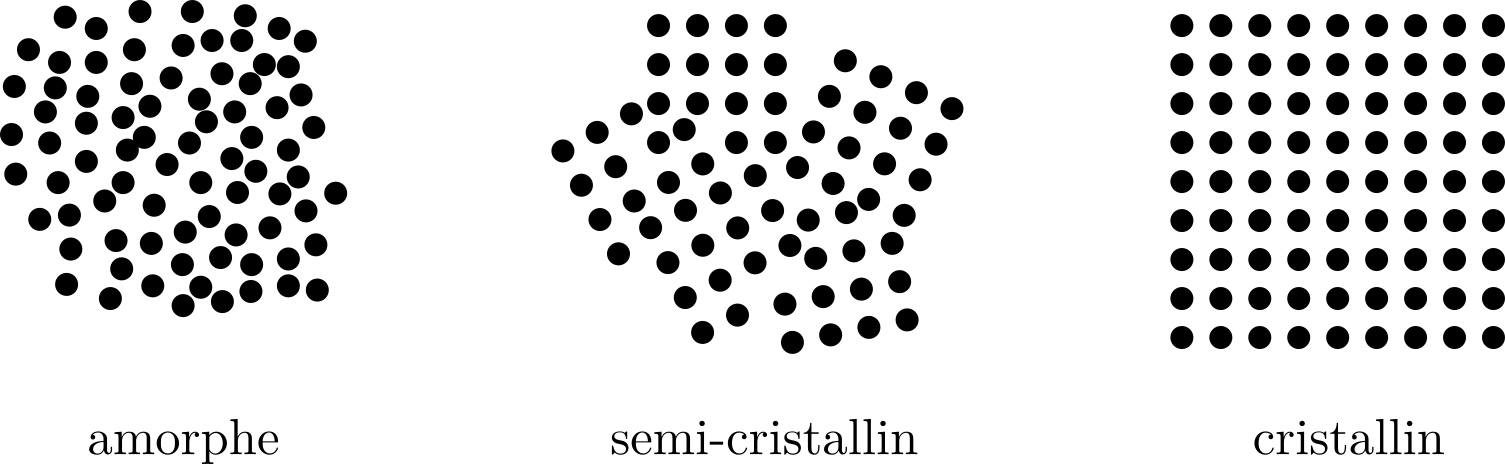
\includegraphics[scale=1]{asc}
	\end{center}
	Les solides amorphes ont une structure microscopique similaire à celle des
	liquides.
	\begin{center}
		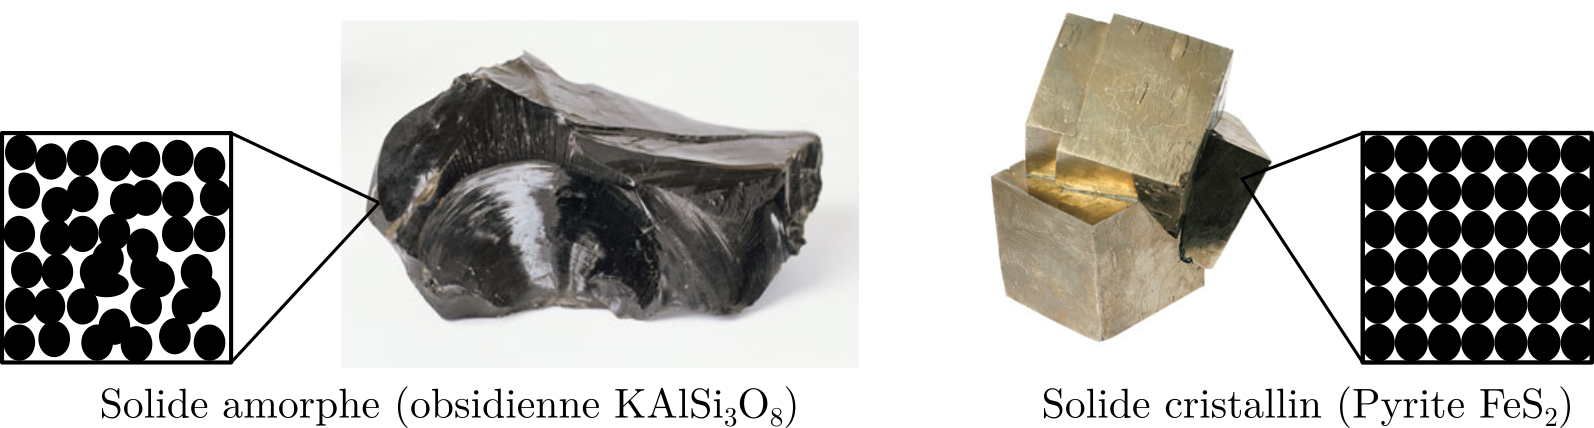
\includegraphics[scale=1]{exem_asc}
	\end{center}
\end{tcb}

Comme pour l'étude des températures d'ébullition dans le chapitre AM2,
l'organisation microscopique se répercute sur les propriétés macroscopiques.
Le but de ce chapitre est de présenter un modèle microscopique simple
permettant l'interprétation de différentes propriétés physiques observables
des solides \textbf{cristallins}.

\subsection{Modèle du cristal parfait de sphères dures}
\subsubsection{Présentation}

\begin{tcb*}(defi){Cristal parfait et sphères dures}
	On modélise un solide cristallin par le modèle théorique du
	\textbf{cristal parfait} constitué de \textbf{sphères dures}~:
	\begin{itemize}
		\item[b]{Cristal parfait}: \psw{structure atomique parfaitement ordonnée
			et infiniment périodique dans l'espace}
		\item[b]{Sphères dures}: \psw{entités constituantes modélisées par des
			sphères dures, impénétrables, indéformables}
	\end{itemize}
\end{tcb*}
C'est évidemment un modèle théorique. Il ne peut être vérifié que sur une
partie du solide, jamais sur sa totalité (notamment sur le bord).

\subsubsection{Description}
Ainsi, pour décrire un cristal, il suffit de trouver un motif à répéter dans
les trois directions de l'espace. On décompose cette répétition basée sur 3
éléments~:
\begin{tcb}(defi){Description d'un cristal}
	\begin{itemize}
		\item[b]{Motif}: la plus petite entité (un atome, un ou plusieurs ions)
		menant à la construction du cristal par translations selon des vecteurs
		de base $\af$, $\bf$ et $\cf$~;
		\item[b]{Réseau}: ensemble des points (appelés \textbf{nœuds}) obtenus par
		translations selon les vecteurs de base~;
		\item[b]{Maille}: l'unité de pavage élémentaire de l'espace~: c'est une
		\textbf{collection de motifs} en 3D.
	\end{itemize}
\end{tcb}

\begin{tcb}(exem)<lftt>{Exemples de motifs}
	\begin{itemize}
		\item[b]{Fer solide}: \psw{atome \ce{Fe}}
		\item[b]{Glace d'eau}: \psw{molécule \ce{H2O}}
		\item[b]{Sel de table}: \psw{deux ions \ce{Na^{+}} et \ce{Cl^{-}}}
	\end{itemize}
\end{tcb}

\begin{tcb}[sidebyside](exem)<lftt>{Réseau, motif et maille}
	\begin{center}
		\sswitch{
			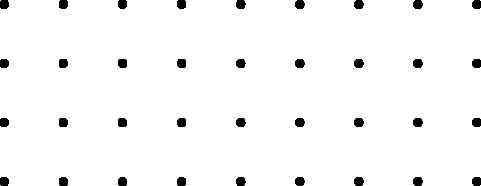
\includegraphics[scale=1]{maille_gen-stud}
		}{
			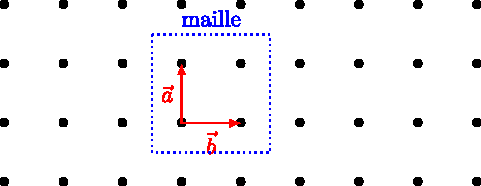
\includegraphics[scale=1]{maille_gen}
		}
		\captionof{figure}{Réseau, motif et maille cubique en 2D.}
	\end{center}
	\tcblower
	\begin{center}
		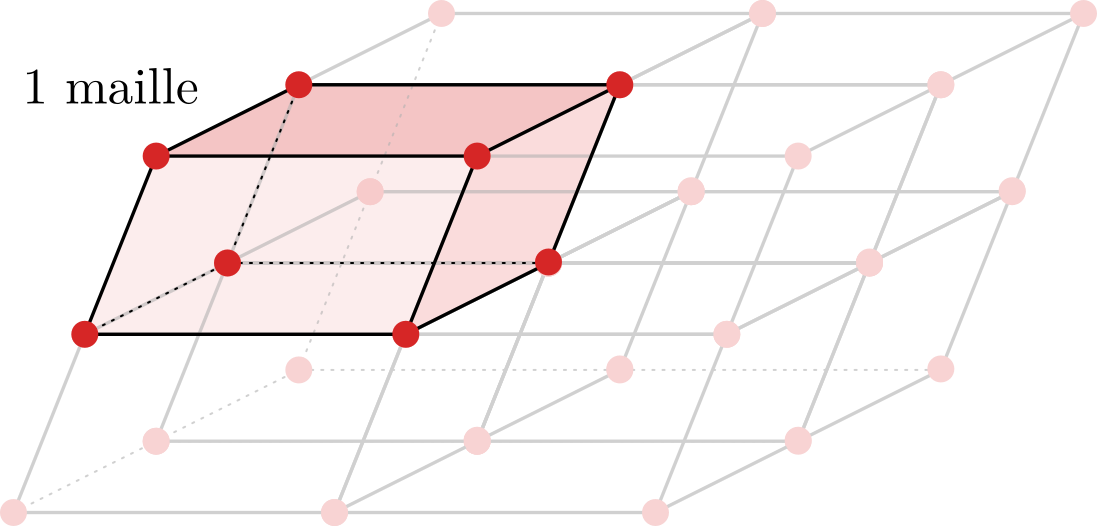
\includegraphics[width=1\linewidth]{maille_paral}
		\captionof{figure}{Réseau, motif et maille parallélépipédique en 3D.}
	\end{center}
\end{tcb}

\begin{tcb*}(prop){Condition de contact}
	Dans une maille, les sphères dures \textbf{les plus proches} sont en contact.
	\begin{center}
		\sswitch{
			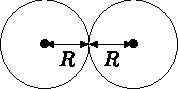
\includegraphics[scale=1, draft=true]{cond_contact}
		}{
			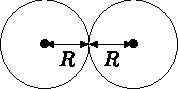
\includegraphics[scale=1]{cond_contact}
		}
	\end{center}
\end{tcb*}

\subsubsection{Limite du cristal parfait}
En réalité, un cristal a des défauts~:
\begin{center}
	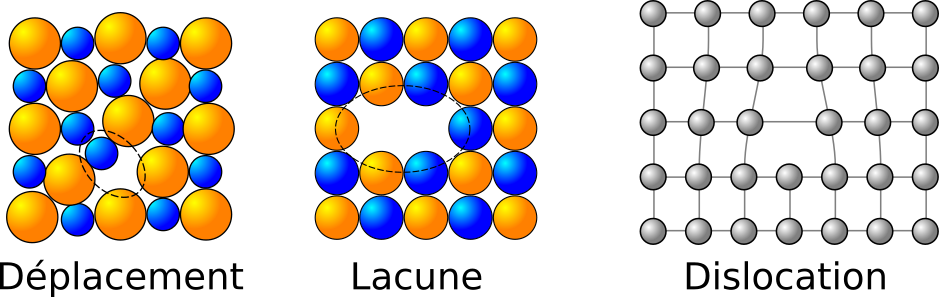
\includegraphics[scale=1]{crist_defaut}
\end{center}
De plus un cristal réel n'est pas infini, il y aura des effets de bords.

\section{Caractérisation des mailles classiques}
\subsection{Vocabulaire}
\begin{tcb}(defi){Caractéristiques d'une maille}
	La maille d'un cristal se caractérise par~:
	\begin{itemize}
		\item[b]{Population} $N$~: \psw{nombre d'entités «~en propre~» par maille}
		\item[b]{Coordinence}: \psw{nombre de plus proches voisins d'une entité}
		\item[b]{Rayon de l'entité}: \psw{rayon maximal qu'une entité peut occuper}
		\item[b]{Compacité}: \psw{pourcentage de l'espace occupé}
		\item[b]{Masse volumique}
	\end{itemize}
\end{tcb}

Pour une visualisation des paramètres de maille,
voir~\url{https://www.ensciences.fr/animations/cristallo/index.html}.

\begin{tcb*}(ror){Caractéristiques d'une maille}
	\begin{itemize}
		\item[b]{Population} $N$~: une entité partagée entre $n$ maille ne compte que
		pour $1/n$. On peut rencontrer les cas suivants~:
		\begin{tasks}[label=\bdmd](4)
			\task\textbf{Sommet}~: \psw{1/8}
			\task\textbf{Arête}~: \psw{1/4}
			\task\textbf{Face}~: \psw{1/2}
			\task\textbf{Volume}~: \psw{1}
		\end{tasks}
		% \begin{itemize}
		% 	\item[b]{Sommet}: \psw{1/8}
		% 	\item[b]{Arête}: \psw{1/4}
		% 	\item[b]{Face}: \psw{1/2}
		% 	\item[b]{Dans le volume}: \psw{1}
		% \end{itemize}
		\item[b]{Coordinence}: il faut faire attention à bien comprendre qu'une maille
		se répète à l'infini dans ce modèle. Ainsi, pour compter les plus proches
		voisins, il faut envisager ceux des mailles adjacentes, non représentées.
		\item[b]{Rayon}: selon le type de cristal (voir plus loin), ça pourra être un
		rayon atomique, un rayon ionique, un rayon covalent ou un rayon de
		\textsc{van der Waals}. On l'obtient par la \textbf{condition de contact/de
			tangence}.
		\item[b]{Compacité}~: notée $C$, on a
		\psw{%
			\[
				\boxed{
					C =
					\frac{\text{volume \textbf{des} motifs}}{\text{volume d'une maille}} =
					\frac{N \times V\ind{motif}}{V\ind{maille}}
					% \frac{\text{population}\times \text{volume d'\textbf{un}
					% 		motif}}{\text{volume d'une maille}}
					<
					1
				}
			\]
		}%
		\vspace{-15pt}
		\item[b]{Masse volumique}: notée $\rho$, on a\ftn{S'il y a plusieurs entités
			de populations différentes, on somme toute la masse de ce qui est en
			propre dans la maille~: $\sum_i N_i M_i$.}
		\psw{%
			\[
				\boxed{
					\rho =
					\frac{\text{masse \textbf{des} motifs}}{\text{volume d'une maille}} =
					\frac{N \times m\ind{motif}}{V\ind{maille}} =
					% \frac{\text{population}\times \text{masse d'\textbf{un}
					% 		motif}}{\text{volume d'une maille}}
					\frac{NM\ind{motif}}{\Nc_AV\ind{maille}}
				}
			\]
		}%
		\vspace{-15pt}
	\end{itemize}
\end{tcb*}

% \subsection{Rappels de la géométrie du cube}
\begin{tcb*}(impo){Dessiner des mailles cubiques}
	Si les mailles seront toutes représentées ici par souci de visualisation, il
	est \textbf{nécessaire} de savoir dessiner une maille~! Pour cela, il est
	utile pour les cubes de placer le sommet «~au fond à gauche~» à $\approx 4/3$
	de la hauteur de la face avant, et $1/3$ ou $2/3$ de sa largeur. Quoi qu'il en
	soit, \textbf{il faut absolument éviter la moitié}~!
\end{tcb*}

\begin{tcb*}[sidebyside, righthand ratio=.3](rapp){Géométrie du cube}
	Dans un cube de côté $a$, on a~:
	\begin{itemize}
		\item 6 faces, 8 sommets et 12 arêtes~;
		\item l'aire d'une face est $a^2$ et le volume $a^3$~;
		      \setlength{\fboxsep}{3mm}
		\item la diagonale $d$ d'une face est $\boxed{\psw{a \sqrt{2}}}$
		\item la diagonale $D$ du cube est $\boxed{\psw{a \sqrt{3}}}$
	\end{itemize}
	\tcblower
	\begin{center}
		\sswitch{
			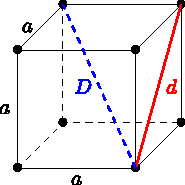
\includegraphics[width=\linewidth, draft=true]{rapp_cube}
		}{
			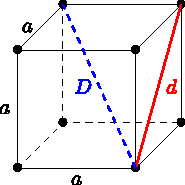
\includegraphics[width=\linewidth]{rapp_cube}
		}
		\vspace{-15pt}
		\captionof{figure}{Schéma.}
	\end{center}
\end{tcb*}

\subsection{Empilements non compacts}
\subsubsection{Maille cubique simple}

Dans un plan, les centres des sphères dures sont réparties selon un pavage
carré. Les différents plans sont exactement superposés les uns aux
autres. On parle parfois d'empilement AAA, mais on le rencontre rarement en
pratique.

\noindent
\begin{tabularx}{\linewidth}{YYY}
	\textbf{Vue de côté}
	 &
	\textbf{Vue du dessus}
	 &
	\textbf{Vue du dessus simplifiée}
	\\
	\begin{center}
		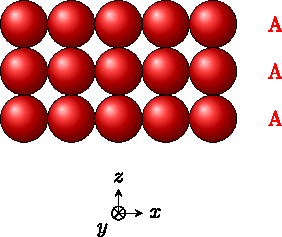
\includegraphics[height=3cm]{emp_AAA_1}
	\end{center}
	 &
	\begin{center}
		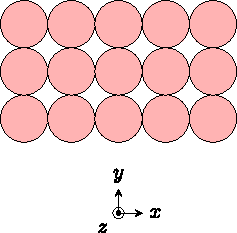
\includegraphics[height=3cm]{emp_AAA_2}
	\end{center}
	 &
	\begin{center}
		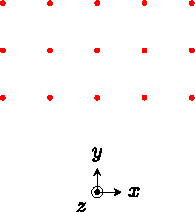
\includegraphics[height=3cm]{emp_AAA_3}
	\end{center}
\end{tabularx}

\begin{tcb*}[breakable](appl)<lftt>{Maille cubique simple}
	\noindent
	\begin{minipage}[t]{.75\linewidth}
		\begin{itemize}
			\item[b]{Population}: \psw{8 atomes sur les sommets, soit
				\[
					N = 8 \times \frac{1}{8} = 1
				\]
			}%
			\vspace{-15pt}
			\item[b]{Coordinence}: \psw{chaque atome voit les voisins sur \textbf{les
					arêtes}, on a donc une coordinence de \textbf{6}}
		\end{itemize}
	\end{minipage}
	\hfill
	\begin{minipage}[t]{.20\linewidth}
		\vspace{0pt}
		\begin{center}
			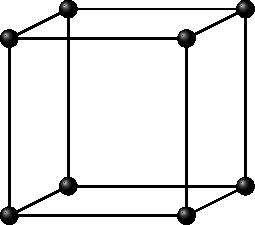
\includegraphics[width=\linewidth]{maille_CS}
		\end{center}
	\end{minipage}
	\begin{itemize}
		\item[b]{Rayon atomique}: \psw{on a tangence \textbf{sur une arête}, soit
			\[
				\boxed{2r = a}
			\]
		}%
		\vspace{-15pt}
		\item[b]{Compacité}:
		\leavevmode\vspace*{-25pt}\relax
		\psw{%
			\begin{gather*}
				C =
				\frac{NV_1}{V} =
				\frac{1 \times \frac{4}{3}\pi r^3}{(2r)^3} =
				\frac{\cancel{4}}{3}\pi \frac{\bcancel{r^3}}{2 \times \cancel{4}
					\bcancel{r^3}}
				\\\Lra
				\boxed{C = \frac{\pi}{6} \approx \num{0.52}}
			\end{gather*}
		}%
		\item[b]{Masse volumique}:
		\leavevmode\vspace*{-25pt}\relax
		\psw{%
			\begin{gather*}
				\rho = \frac{M}{\Nc_A \times a^3}
			\end{gather*}
		}%
	\end{itemize}
\end{tcb*}

\subsubsection{Maille cubique centrée}
On dispose une entité en plus au centre de la maille cubique simple~:
\begin{tcb*}[breakable](appl)<lftt>{Maille cubique centrée}
	\noindent
	\begin{minipage}[t]{.75\linewidth}
		\begin{itemize}
			\item[b]{Population}: \psw{8 atomes sur les sommets et 1 au centre, soit
				\[
					N = 8 \times \frac{1}{8} + 1 = 2
				\]
			}%
			\vspace{-15pt}
			\item[b]{Coordinence}: \psw{chaque atome voit les voisins sur \textbf{les
					sommets}, on a donc une coordinence de \textbf{8}}
		\end{itemize}
	\end{minipage}
	\hfill
	\begin{minipage}[t]{.20\linewidth}
		\vspace{0pt}
		\begin{center}
			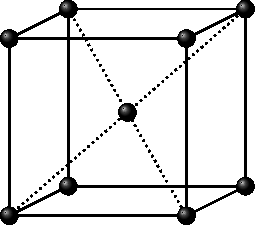
\includegraphics[width=\linewidth]{maille_CC}
		\end{center}
	\end{minipage}
	\begin{itemize}
		\item[b]{Rayon atomique}: \psw{on a tangence \textbf{sur la grande
				diagonale}, soit
			\[
				r + 2r + r = a \sqrt{3} \Lra \boxed{\frac{4r}{\sqrt{3}} = a}
			\]
		}%
		\vspace{-15pt}
		\item[b]{Compacité}:
		\leavevmode\vspace*{-25pt}\relax
		\psw{%
			\begin{gather*}
				C =
				\frac{NV_1}{V} =
				\frac{2 \times \frac{\bcancel{4}}{\cancel{3}}\pi \dcancel{r^3}}
				{\frac{\bcancel{4} \times 16}{\cancel{3} \sqrt{3}}\dcancel{r^3}}
				\\\Lra
				\boxed{C = \frac{\sqrt{3}\pi}{8} \approx \num{0.68}}
			\end{gather*}
		}%
		\item[b]{Masse volumique}:
		\leavevmode\vspace*{-25pt}\relax
		\psw{%
			\begin{gather*}
				\rho = \frac{2M}{\Nc_A \times a^3}
			\end{gather*}
		}%
	\end{itemize}
\end{tcb*}

\subsection{Empilements compacts}
Les empilements dits compacts sont ceux qui laissent le moins d'espace
disponible entre les différentes sphères. Décrire ces empilements nécessite non
plus un seul mais trois types de plans d'atomes, appelés A, B et C.
\begin{enumerate}
	\item[b]{Premier plan}: chaque sphère s'entoure de six autres sphères, aux
	sommets d'un hexagone régulier. On l'appelle le plan A.
	\smallbreak
	\noindent
	\begin{tabularx}{\linewidth}{YYY}
		\textbf{Vue de côté}
		 &
		\textbf{Vue du dessus}
		 &
		\textbf{Vue du dessus simplifiée}
		\\
		\begin{center}
			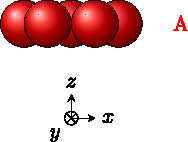
\includegraphics[height=3cm]{emp_A_1}
		\end{center}
		 &
		\begin{center}
			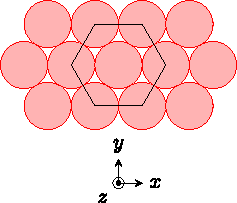
\includegraphics[height=3cm]{emp_A_2}
		\end{center}
		 &
		\begin{center}
			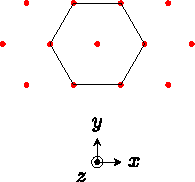
\includegraphics[height=3cm]{emp_A_3}
		\end{center}
	\end{tabularx}
	\item[b]{Deuxième plan}: dans le plan immédiatement supérieur au plan A,
	chaque sphère va se placer dans un des creux des sphères du plan A.
	Cependant, seul un creux sur deux peut être occupé.
	\smallbreak
	\noindent
	\begin{tabularx}{\linewidth}{YYY}
		\textbf{Vue de côté}
		 &
		\textbf{Vue du dessus}
		 &
		\textbf{Vue du dessus simplifiée}
		\\
		\begin{center}
			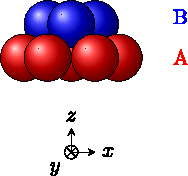
\includegraphics[height=3cm]{emp_AB_1}
		\end{center}
		 &
		\begin{center}
			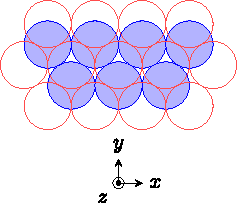
\includegraphics[height=3cm]{emp_AB_2}
		\end{center}
		 &
		\begin{center}
			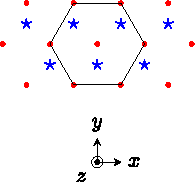
\includegraphics[height=3cm]{emp_AB_3}
		\end{center}
	\end{tabularx}
	\item[b]{Troisième plan}: les sphères du plan immédiatement supérieur au plan
	B se placent à nouveau dans les creux des sphères du plan B, mais il y a
	cette fois deux choix non-équivalents~:
	\begin{itemize}
		\item les sphères se placent dans les cavités de B mais immédiatement
		      au-dessus du plan A~: c'est un nouveau plan A, et on parle d'empilement
		      ABA, ce qui donne la \textbf{maille hexagonale compacte}~;
		      \smallbreak
		      \noindent
		      \begin{tabularx}{\linewidth}{YYY}
			      \textbf{Vue de côté}
			       &
			      \textbf{Vue du dessus}
			       &
			      \textbf{Vue du dessus simplifiée}
			      \\
			      \begin{center}
				      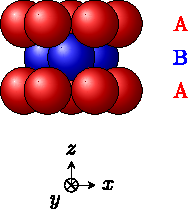
\includegraphics[height=3cm]{emp_ABA_1}
			      \end{center}
			       &
			      \begin{center}
				      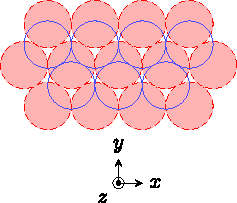
\includegraphics[height=3cm]{emp_ABA_2}
			      \end{center}
			       &
			      \begin{center}
				      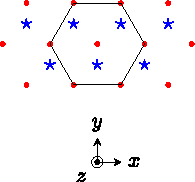
\includegraphics[height=3cm]{emp_ABA_3}
			      \end{center}
		      \end{tabularx}
		\item les sphères se placent dans les cavités de B mais au-dessus des
		      \textbf{creux} de A, ceux que le plan B laissait libre~: c'est un
		      \textbf{nouveau plan}, formant un empilement ABC, ce qui donne la
		      \textbf{maille cubique face centrée}.
		      \smallbreak
		      \noindent
		      \begin{tabularx}{\linewidth}{YYY}
			      \textbf{Vue de côté}
			       &
			      \textbf{Vue du dessus}
			       &
			      \textbf{Vue du dessus simplifiée}
			      \\
			      \begin{center}
				      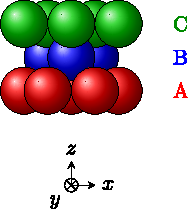
\includegraphics[height=3cm]{emp_ABC_1}
			      \end{center}
			       &
			      \begin{center}
				      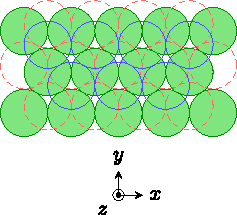
\includegraphics[height=3cm]{emp_ABC_2}
			      \end{center}
			       &
			      \begin{center}
				      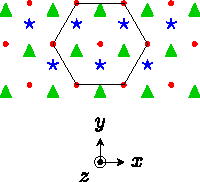
\includegraphics[height=3cm]{emp_ABC_3}
			      \end{center}
		      \end{tabularx}
	\end{itemize}
\end{enumerate}

\subsubsection{Maille hexagonale}
Par exemple, le magnésium, le béryllium, etc.\ cristallisent en hexagonal
compact. La description de cette maille est hors-programme, en particulier aucun
calcul géométrique (compacité, masse volumique) n'est exigible pour cette
maille.
\smallbreak
\begin{isd}[righthand ratio=.20]
	\begin{itemize}
		\item[b]{Population}: \psw{1 atome dans la maille, 8 atomes sur les sommets
			donc
			\[
				N = 1 + 8 \times \frac{1}{8} = 2
			\]
		}%
		\item[b]{Compacité}: on peut montrer qu'elle est de \num{0.74},
		caractéristiques des empilements compacts.
	\end{itemize}
	\tcblower
	\begin{center}
		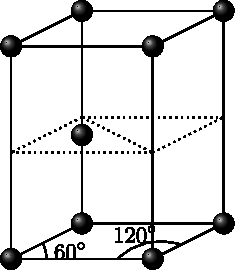
\includegraphics[width=\linewidth]{maille_hc}
	\end{center}
\end{isd}

\subsubsection{Maille cubique face centrée}
\begin{tcb*}[sidebyside, righthand ratio=.25](defi){Maille cubique face centrée}
	La maille cubique face centrée est un cube de coté $a$. On dispose une
	particule à chaque sommet du cube et une particule au milieu de chacune des
	faces. Les particules se touchent sur la \textbf{diagonale d'une face}.
	\tcblower
	\begin{center}
		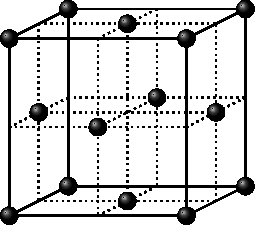
\includegraphics[width=\linewidth]{maille_CFC}
	\end{center}
\end{tcb*}
Cet empilement est celui du cuivre, du nickel, du platine, de l'or, etc.

\begin{tcb*}[breakable](appl)<lftt>{Maille cubique face centrée}
	\noindent
	\begin{minipage}[t]{.72\linewidth}
		\begin{itemize}
			\item[b]{Population}: \psw{8 atomes sur les sommets et 6 sur les faces,
				soit
				\[
					N = 8 \times \frac{1}{8} + 6 \times \frac{1}{2} = 4
				\]
			}%
		\end{itemize}
	\end{minipage}
	\hfill
	\begin{minipage}[t]{.24\linewidth}
		\vspace{0pt}
		\begin{center}
			\sswitch{
				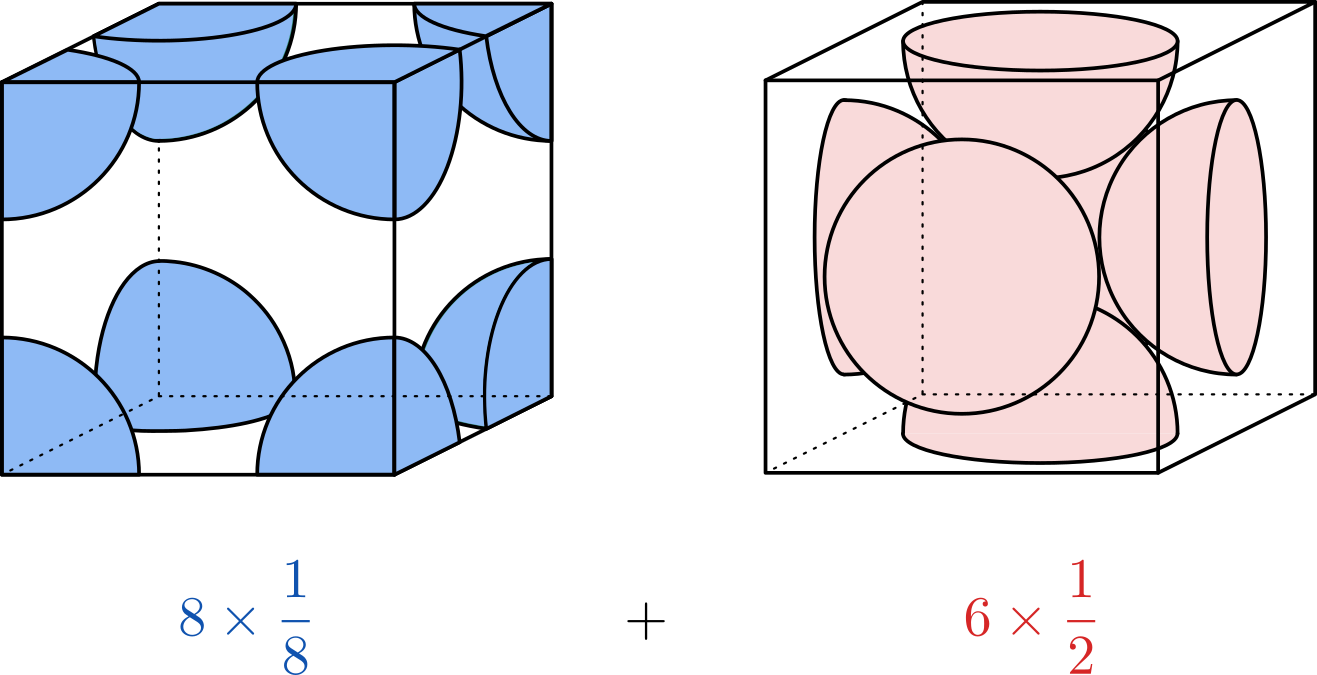
\includegraphics[width=\linewidth, draft=true]{maille_CFC_pop}
			}{
				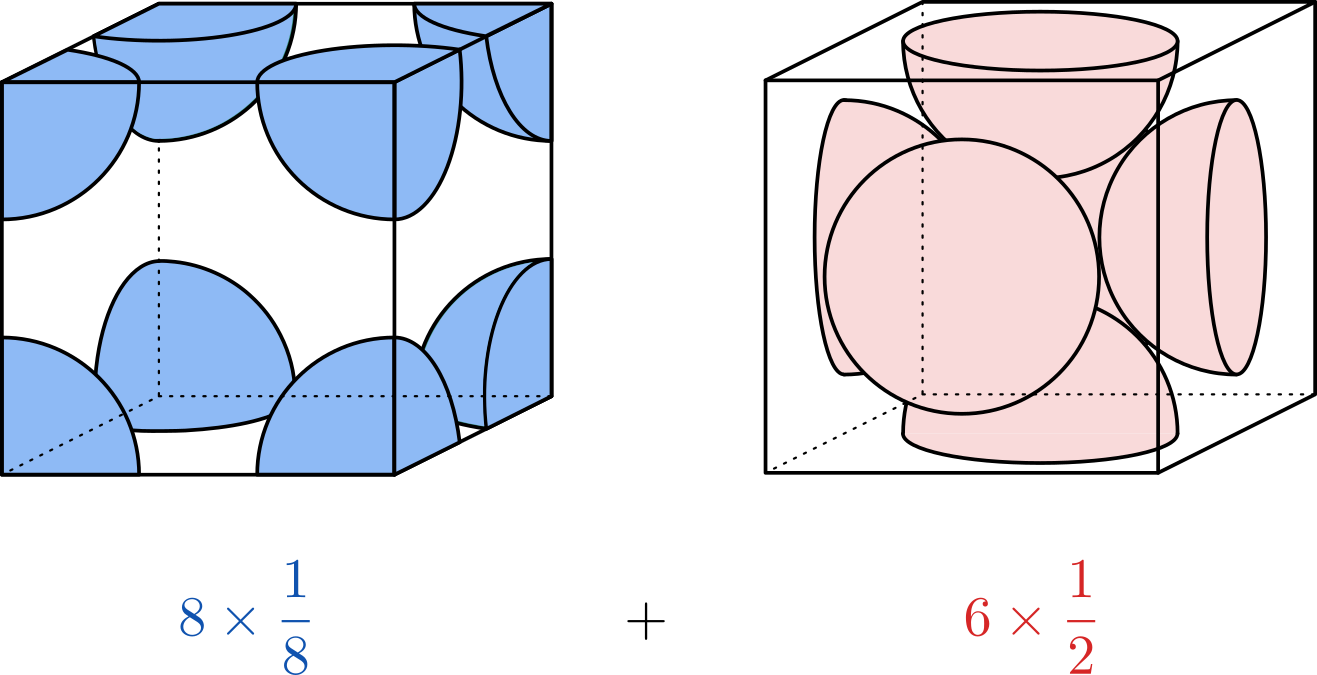
\includegraphics[width=\linewidth]{maille_CFC_pop}
			}
		\end{center}
	\end{minipage}
	\noindent
	\begin{minipage}[t]{.72\linewidth}
		\begin{itemize}
			\item[b]{Coordinence}: \psw{chaque atome voit les voisins sur \textbf{les
					petites diagonales des faces}. Par exemple, l'atome du centre de la
				face supérieure voit les 4 du même plan, les 4 du plan inférieur et
				les 4 du plan au-dessus, non représenté. On a donc une coordinence de
				\textbf{12}, caractéristique d'une maille compacte.}
		\end{itemize}
	\end{minipage}
	\hfill
	\begin{minipage}[t]{.24\linewidth}
		\vspace{0pt}
		\begin{center}
			\sswitch{
				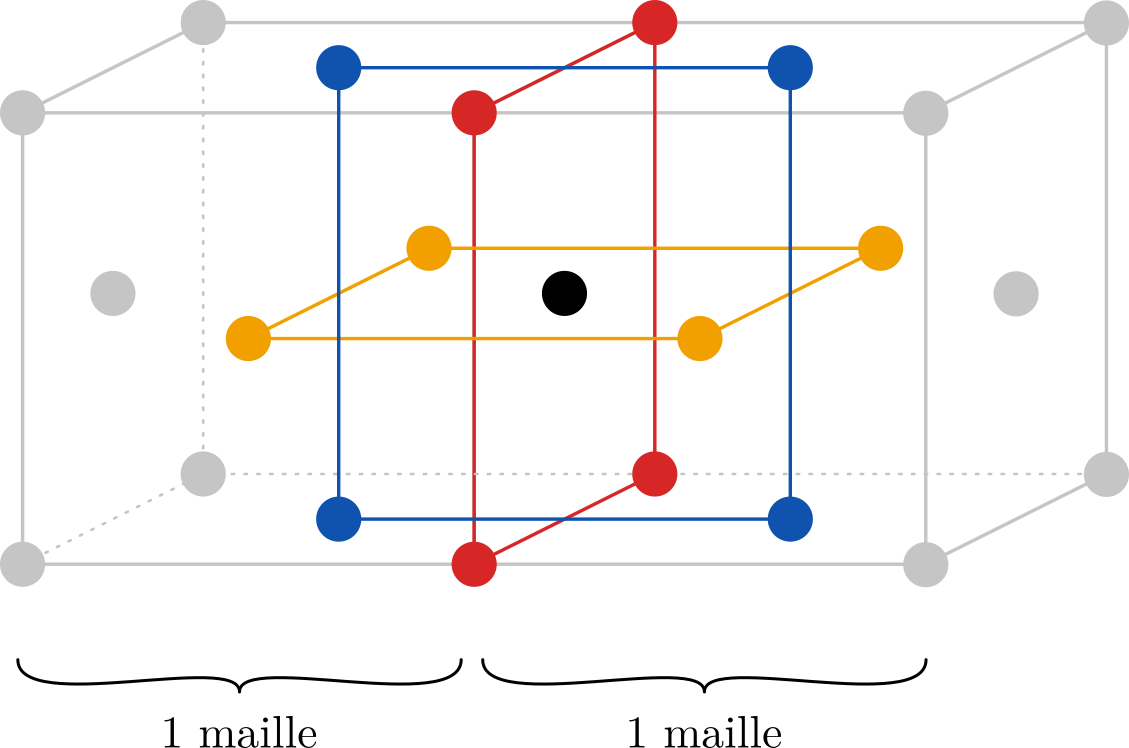
\includegraphics[width=\linewidth, draft=true]{maille_CFC_coord}
			}{
				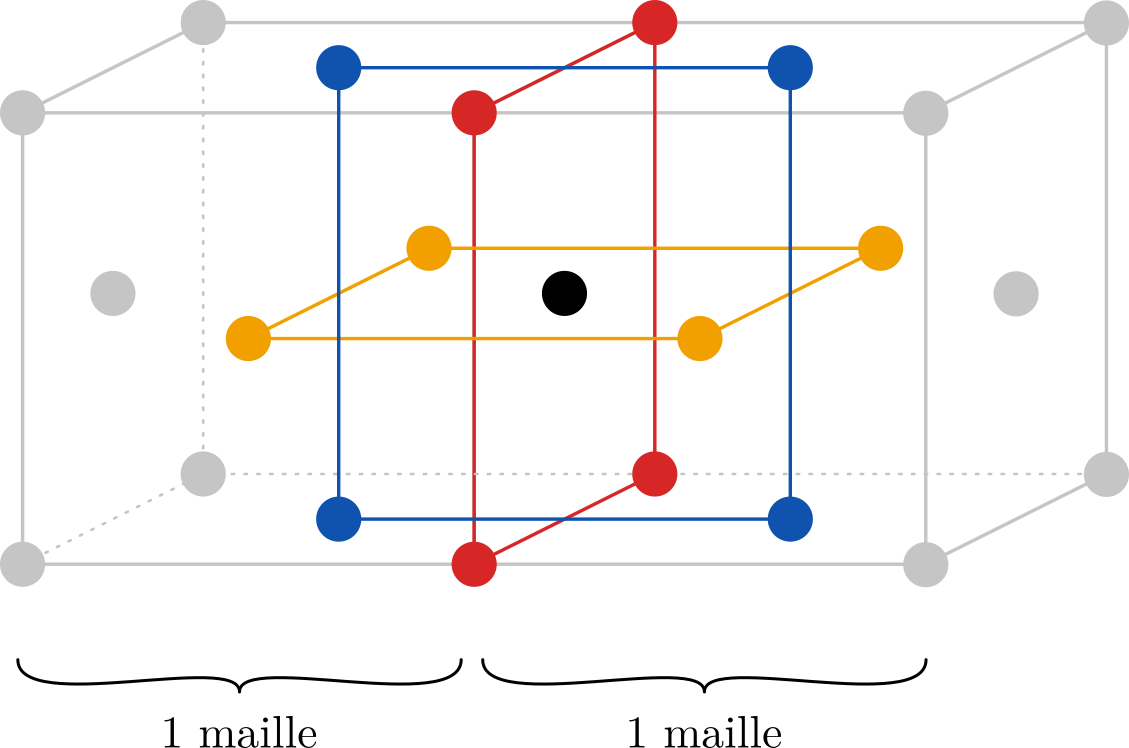
\includegraphics[width=\linewidth]{maille_CFC_coord}
			}
		\end{center}
	\end{minipage}
	\noindent
	\begin{minipage}[t]{.72\linewidth}
		\begin{itemize}
			\item[b]{Rayon atomique}: \psw{on a tangence \textbf{sur les petites
					diagonales}, soit
				\[
					r + 2r + r = a \sqrt{2} \Lra \boxed{2r \sqrt{2} = a}
				\]
			}%
		\end{itemize}
	\end{minipage}
	\hfill
	\begin{minipage}[t]{.24\linewidth}
		\vspace{0pt}
		\begin{center}
			\sswitch{
				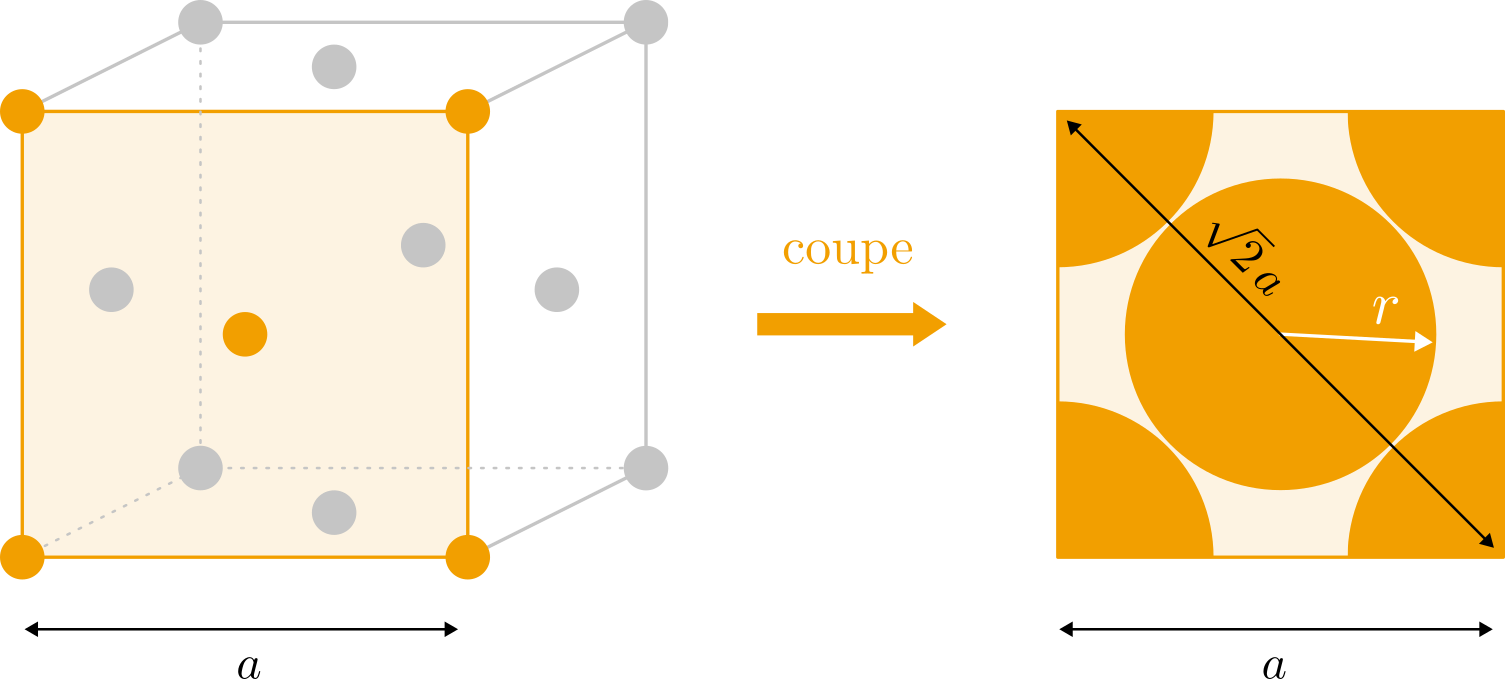
\includegraphics[width=\linewidth, draft=true]{maille_CFC_rayon}
			}{
				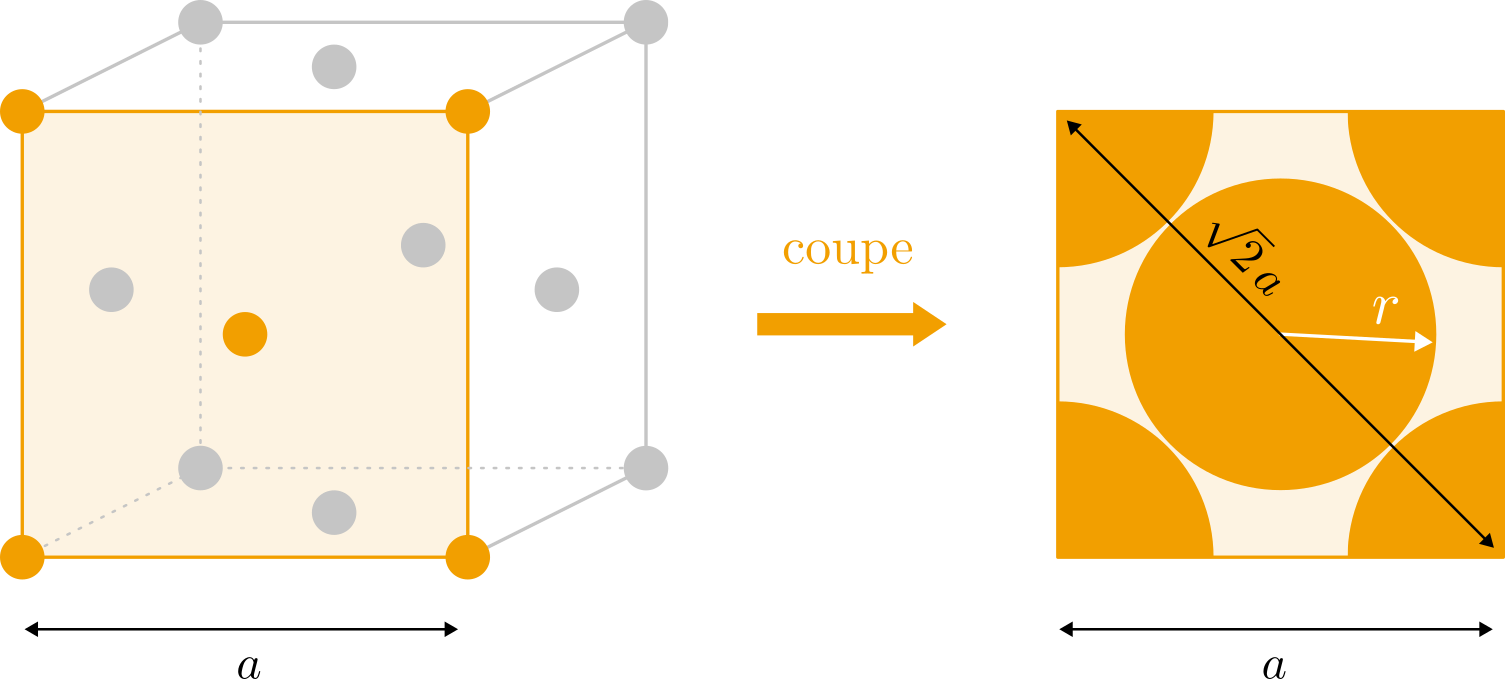
\includegraphics[width=\linewidth]{maille_CFC_rayon}
			}
		\end{center}
	\end{minipage}
	\begin{itemize}
		\item[b]{Compacité}:
		\leavevmode\vspace*{-25pt}\relax
		\psw{%
			\begin{gather*}
				C =
				\frac{NV_1}{V} =
				\frac{\bcancel{4} \times \frac{\bcancel{4}}{3}\pi \cancel{r^3}}
				{\bcancel{16} \sqrt{2}\cancel{r^3}}
				\\\Lra
				\boxed{C = \frac{\pi}{3 \sqrt{2}} \approx \num{0.74}}
			\end{gather*}
		}%
		\item[b]{Masse volumique}: pour le cuivre $a = \SI{128}{pm}$ et $M =
			\SI{64}{g.mol^{-1}}$,
		\psw{%
			\begin{gather*}
				\rho = \frac{4M}{\Nc_A \times a^3} = \SI{8.9e3}{kg.m^{-3}}
			\end{gather*}
		}%
		\vspace{-20pt}
	\end{itemize}
\end{tcb*}

\section{Sites interstitiels CFC}
\subsection{Présentation}
Les structures précédentes, bien que compactes, présentent beaucoup de vide~:
\SI{26}{\%} du volume n'est pas occupé~!
\begin{tcb*}(defi){Sites cristallographiques}
  Les \textbf{sites} (cristallographiques ou interstitiels) sont les
  \textbf{espaces vides où les sphères ne se touchent pas} au sein d'une maille,
  dans lesquels \textbf{de plus petites entités peuvent s'insérer}.
	\smallbreak
	On appelle \textbf{habitabilité} d'un site le \textbf{rayon maximal} d'une
	sphère dure s'y insérant, sans déformer la maille~: on l'obtient par condition
	de tangence avec les sphères du réseau.
\end{tcb*}

Les empilements AB font apparaître deux types de sites~:
\begin{center}
	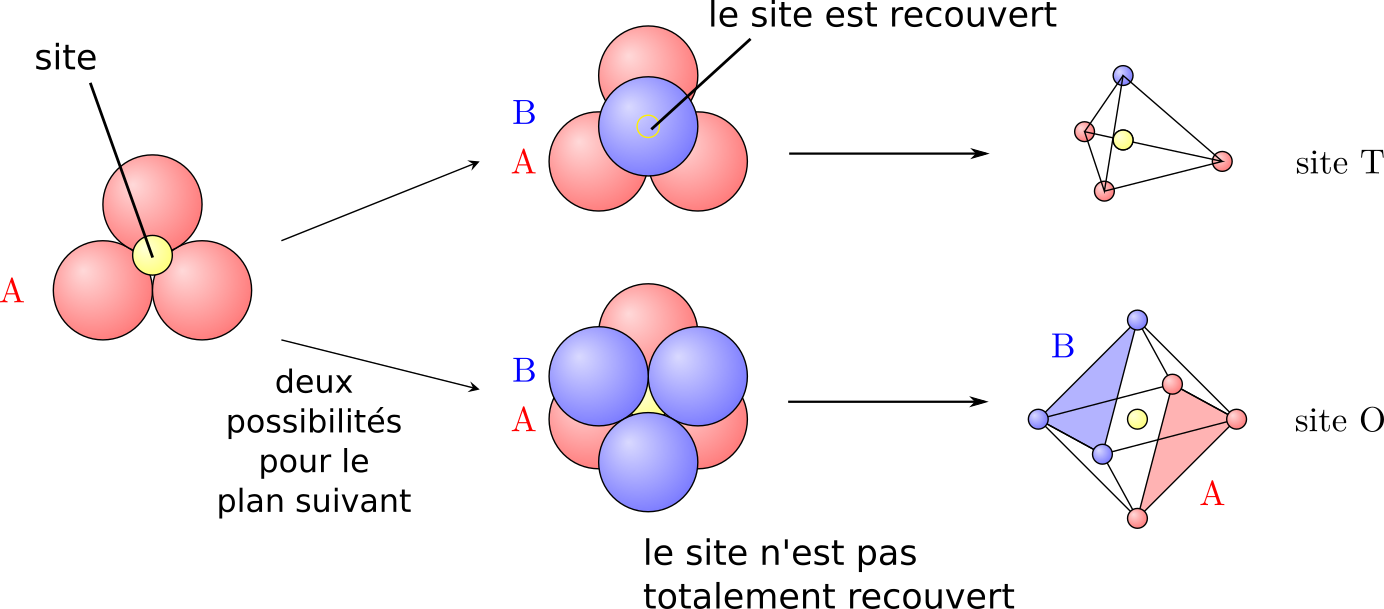
\includegraphics[scale=1]{sites_pres}
\end{center}

\subsection{Sites tétraédriques}
\begin{tcb*}(prop){Sites tétraédriques}
	Les sites tétraédriques se situent au \textbf{centre des petits cubes} de côté
	$a/2$. Ils ont 4 plus proches voisins, et forment donc un \textbf{tétraèdre
		régulier}.
	\smallbreak
	\begin{isd}
		\begin{center}
			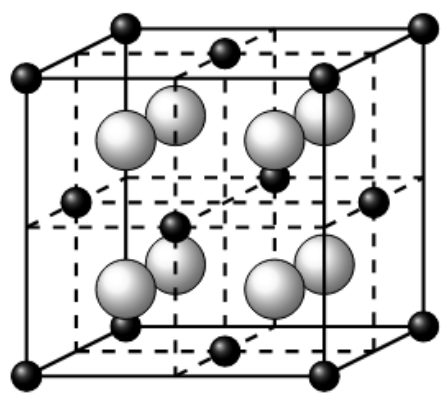
\includegraphics[scale=1]{sites_T-8.png}
		\end{center}
		\tcblower
		\begin{center}
			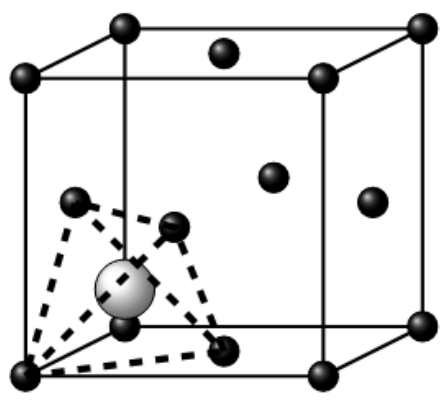
\includegraphics[scale=1]{sites_T-1.png}
		\end{center}
	\end{isd}
\end{tcb*}

\begin{tcb*}[breakable](appl)<lftt>{Sites tétraédriques}
	\begin{isd}[righthand ratio=.25]
		\begin{enumerate}[label=\sqenumi]
			\item Déterminer $N_T$ la population de sites T par maille.
			\item Déterminer l'habitabilité $r_T$ en fonction de $a$ et $r$.
			\item Exprimer $r_T$ en fonction de $r$ seulement. Commenter.
		\end{enumerate}
		\tcblower
		\begin{center}
			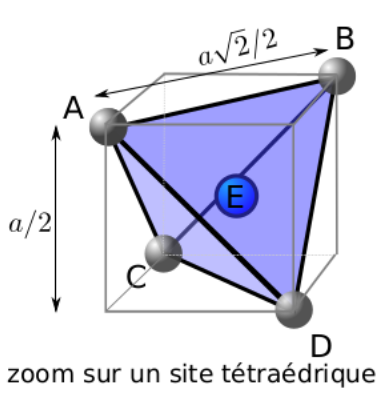
\includegraphics[width=\linewidth]{site_T_zoom.png}
		\end{center}
	\end{isd}
	\tcblower
	\begin{enumerate}[label=\sqenumi]
		\item \psw{On a 8 sites dans le volume, soit $N_T = \num{8}$.}
		\item
		      \psw{%
			      On a tangence \textbf{sur la moitié de la diagonale du petit
				      cube}~:
			      \begin{gather*}
				      r + r_T = \frac{a \sqrt{3}}{4}
				      \Lra
				      \boxed{r_T = \frac{a \sqrt{3}}{4} - r}
			      \end{gather*}
		      }%
		      \vspace{-15pt}
		\item
		      \psw{%
			      Or, dans la maille principale, on a tangence sur la diagonale
			      d'une face, donc $a = 2r \sqrt{2}$. Ainsi,
			      \[
				      \boxed{r_T = \left( \sqrt{\frac{3}{2}} - 1 \right)r \approx \num{0.225}r}
			      \]
			      Pour pouvoir insérer un élément dans un site tétraédrique sans
			      déformer le réseau, il faut que son rayon soit inférieur ou égal à
			      $\num{0.225}r$~: il faut donc une entité \xul{5 fois plus petite}.
		      }%
	\end{enumerate}
\end{tcb*}

\subsection{Sites octaédriques}
\begin{tcb*}(prop){Sites octaédriques}
	Les sites octaédriques se situent au \textbf{centre de la maille} ainsi
	qu'\textbf{au milieu des arêtes}. Ils ont 6 plus proches voisins, et forment
	donc un \textbf{octaèdre régulier}.
	\smallbreak
	\begin{isd}
		\begin{center}
			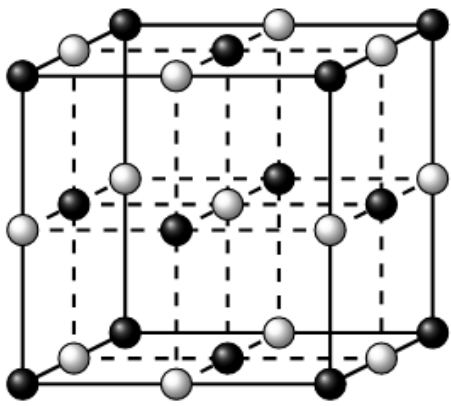
\includegraphics[scale=1]{sites_O-4.png}
		\end{center}
		\tcblower
		\begin{center}
			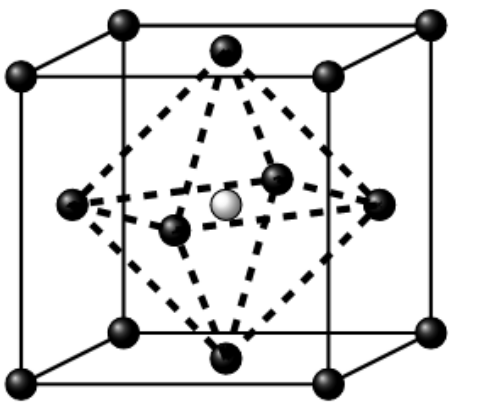
\includegraphics[scale=1]{sites_O-1.png}
		\end{center}
	\end{isd}
\end{tcb*}

\begin{tcb*}[breakable](appl)<lftt>{Sites octaédriques}
	\begin{isd}[righthand ratio=.25]
		\begin{enumerate}[label=\sqenumi]
			\item Déterminer $N_O$ la population de sites O par maille.
			\item Déterminer l'habitabilité $r_O$ en fonction de $a$ et $r$.
			\item Exprimer $r_O$ en fonction de $r$ seulement. Commenter.
		\end{enumerate}
		\tcblower
		\begin{center}
			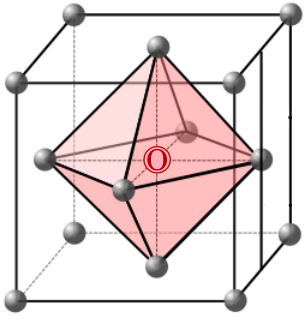
\includegraphics[width=\linewidth]{site_O_zoom.png}
		\end{center}
	\end{isd}
	\tcblower
	\begin{enumerate}[label=\sqenumi]
		\item
		      \psw{%
			      On a 12 sites sur les arêtes et 1 dans le volume, soit $N_O = 1 +
				      12 \times \frac{1}{4} = \num{4}$.
		      }%
		\item
		      \psw{%
			      On a tangence \textbf{sur une arête}~:
			      \begin{gather*}
				      2(r + r_O) = a
				      \Lra
				      \boxed{r_O = \frac{a}{2} - r}
			      \end{gather*}
		      }%
		\item
		      \psw{%
			      Or, dans la maille principale, on a tangence sur la diagonale
			      d'une face, donc $a = 2r \sqrt{2}$. Ainsi,
			      \[
				      \boxed{r_O = \left( \sqrt{2} - 1 \right)r \approx \num{0.414}r}
			      \]
			      Pour pouvoir insérer un élément dans un site tétraédrique sans
			      déformer le réseau, il faut que son rayon soit inférieur ou égal à
			      $\num{0.414}r$~: il faut donc une entité \xul{2 fois plus petite}.
		      }%
	\end{enumerate}
\end{tcb*}
\section{Différents types de cristaux}
\begin{tcb*}[list entry={\lte Propriétés macro.\ des solides}](defi){Propriétés macroscopiques des solides}
	Les solides cristallins présentent des propriétés macroscopiques très
	diversifiées. Par exemple, mécaniquement on distingue~:
	\begin{itemize}
		\item la \textbf{dureté}~: \psw{résistance à la pénétration~;}
		\item la \textbf{malléabilité}~: \psw{capacité à se déformer (par choc ou
			      pression) sans rompre~;}
		\item la \textbf{ductilité}~: \psw{capacité à être étiré sans casser.}
	\end{itemize}
	On trouve également des propriétés \textbf{électriques} et \textbf{chimiques}
	(solubilité, température de fusion).
\end{tcb*}

On peut alors les regrouper par famille, selon leur structure microscopique dont
émergent les propriétés macro~: c'est l'objectif des paragraphes suivants.

\subsection{Cristaux métalliques}
\subsubsection{Description}
\begin{tcb*}[sidebyside, righthand ratio=.4](defi){Modèle des métaux}
	On peut décrire un cristal métallique comme une structure dans laquelle les
	nœuds du réseau sont occupés par des \textbf{cations} (\ce{M+} ou \ce{M^{2+}},
	perte d'un ou deux électrons de valence), et tous les électrons cédés sont
	\textbf{délocalisés} sur l'ensemble du cristal. Cette délocalisation assure la
	cohésion du cristal.
	\tcblower
	\begin{center}
		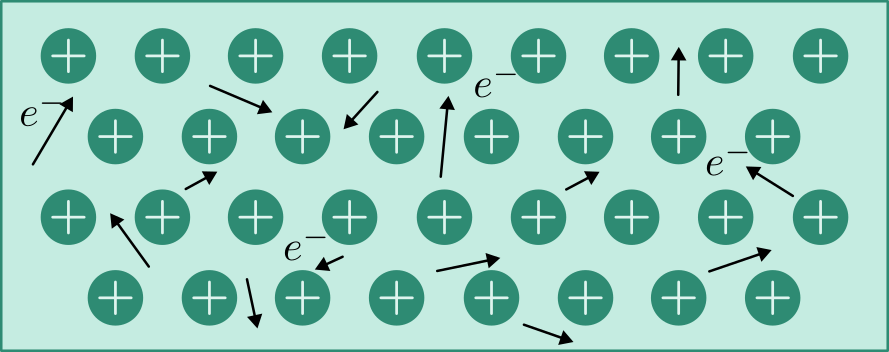
\includegraphics[width=\linewidth]{metal_mod}
	\end{center}
\end{tcb*}

\begin{tcb}(rema)<lftt>{Classification périodique}
	Conventionnellement, la limite entre métaux et non-métaux est définie comme
	sur la figure ci-après, mais elle est relativement floue. Entre les deux, on
	a les semi-conducteurs (ou métalloïdes, ou semi-métaux), qui ont des
	propriétés métalliques peu marquées.
	\begin{center}
		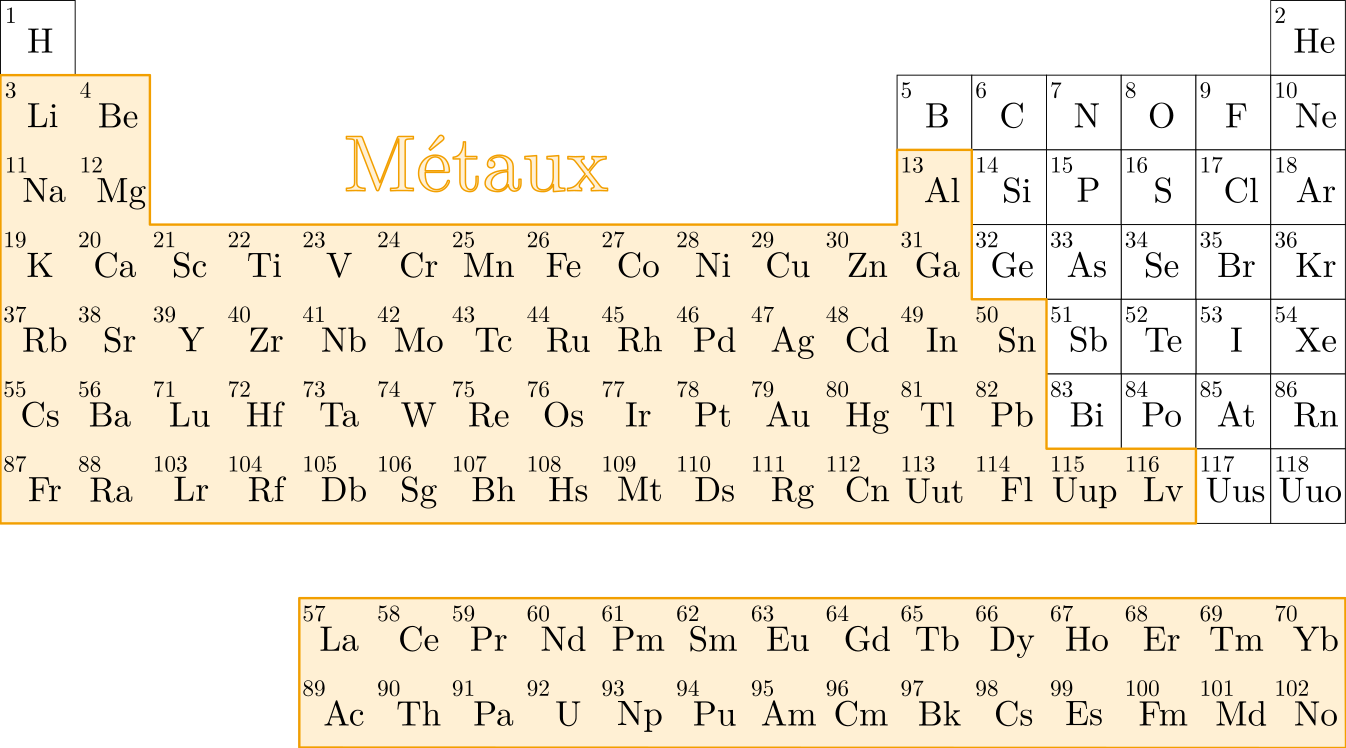
\includegraphics[scale=1]{metaux}
	\end{center}
\end{tcb}

% \begin{tcb*}(prop){Liaison métallique}
% 	\psw{
% 		\begin{center}
%       La liaison métallique est \textbf{forte} ($E \approx
%       \SI{100}{kJ.mol^{-1}}$) et \textbf{isotrope}/non-directionnelle (égale
%       dans toutes les directions).
% 		\end{center}
% 	}
% \end{tcb*}
%
% \begin{tcb*}(prop){Électronégativité des métaux}
% 	\psw{
% 		\begin{center}
% 			Un métal est un élément \textbf{peu électronégatif}.
% 		\end{center}
% 	}
% \end{tcb*}

\def\rght{0.750}
L'étude de leurs propriétés microscopique permet d'expliquer leurs propriétés
macroscopiques~:
\begin{tcb*}[tabularx={lXcY}, label=ror:ptemet](ror){Propriétés des métaux}
	\\[-0.5em]
	\textbf{Type}                                                                &
	\multicolumn{1}{Y}{%
		\textbf{Ppté.\ microscopique}}                                               &       &
	\textbf{Ppté.\ macroscopique}
	\\\midrule
	\textbf{Mécanique}                                                           &
	Liaison isotrope donc atomes déplaçables                                     & $\Ra$ &
	\psw{ductile et malléable}
	\\\midrule
	\textbf{Thermique}                                                           &
	Liaison métallique forte\ftn{%
		$\Ec\ind{métal} \approx \SI{100}{kJ.mol^{-1}}$}
	$\xmathstrut{\rght}$
	& $\Ra$ &
	\psw{température de fusion élevée}
	\\\midrule
	\textbf{Électrique}                                                          &
	Électrons libres
	$\xmathstrut{\rght}$
	& $\Ra$ &
	\psw{conductivité électrique et thermique}
	\\\midrule
	\textbf{Chimique}                                                            &
	Électrons facilement arrachés ($\chi \searrow$)
	$\xmathstrut{\rght}$
	& $\Ra$ &
	\psw{métaux réducteurs}
	\\\bottomrule
\end{tcb*}

% \begin{tcb*}(ror){Propriétés des métaux}
%   \begin{itemize}
%     \item[b]{Mécanique}: \psw{ductiles}
%     \item[b]{Thermique}: \psw{bons conducteurs thermiques}
%   \end{itemize}
%
% \end{tcb*}


\subsubsection{Alliages métalliques}
\begin{tcb}(defi){Définition}
	\begin{center}
		Un alliage est un cristal combinant un métal (dit \textit{de base}) avec
		un ou plusieurs autres éléments (dits \textit{d'alliage}), métalliques
		ou non.
	\end{center}
\end{tcb}

On dit aussi parfois qu'un alliage est une «~solution solide~»~: la base serait
le solvant, les autres les solutés. L'intérêt des alliages est de faire varier
les propriétés du matériau de base, notamment mécaniques et anti-corrosives. On
peut les réaliser de deux manières~:
\begin{enumerate}
	\item par \textbf{substitution}~: un atome se substitue à un autre en certains
	      points du réseau~;
	\item par \textbf{insertion}~: des atomes s'insèrent dans les sites
	      cristallographiques du réseau métallique.
\end{enumerate}

\begin{table}[ht]
	\footnotesize
	\renewcommand\arraystretch{1.3}
	\caption{Exemples d'alliages courants et utilisations}
	\label{tab:alliages}
	\begin{tabularx}{\linewidth}{YYYm{8cm}}
		\toprule
		\textbf{Nom de l'alliage} & \textbf{Élément principal} & \textbf{Éléments
		ajoutés}                  &
		\multicolumn{1}{>{\centering\arraybackslash}m{7cm}}{\textbf{Propriétés et
			utilisations}}
		\\\midrule
		Acier                     & Fer                        & Carbone 2\%                   & Plus dur que le fer. Très répandu, notamment en
		construction ou dans l'industrie automobile.
		\\
		Acier inoxydable          & Fer                        & Carbone 2\%, chrome et nickel & Plus résistant à
		la corrosion que l'acier simple.
		\\
		Alliages d'aluminium      & Aluminium                  & Cobalt, nickel, tantale       & Alliages durs
		mais légers, utilisés notamment en aéronautique.
		\\
		Bronze                    & Cuivre > 60\%              & Étain                         & Plus résistant que le cuivre à l'usure.
		Utilisé pour la décoration , la lutherie, la sculpture.
		\\
		Laiton                    & Cuivre > 60\%              & Zinc                          & Plus dur et plus facile à usiner que le
		cuivre. Utilisé en horlogerie, serrurerie, robinetterie, lutherie.
		\\
		Or rose                   & Or                         & Cuivre 20\%, argent 5\%       & Utilisé en joaillerie.
		\\
		Or blanc                  & Or                         & Argent                        & Utilisé en joaillerie, recouvert d'une couche de
		rhodium pour le rendre plus brillant.
		\\\bottomrule
	\end{tabularx}
\end{table}

\subsection{Cristaux ioniques}
\subsubsection{Description}
\begin{tcb*}(defi){Cristal ionique}
	\psw{
		\begin{center}
			Un cristal ionique est un assemblage \textbf{électriquement neutre} de
			cations et d'anions.
		\end{center}
	}
\end{tcb*}
\begin{tcb}(appl)<lftt>'l'{Formule brute d'un cristal}
	Déterminer la formule brute d'un cristal contenant les ions \ce{Fe^{3+}} et
	\ce{O^{2-}}.
	\tcblower
	\psw{
		Pour avoir neutralité, pour chaque cation \ce{Fe^{3+}} on doit avoir un nombre
		d'anion \ce{O^{2-}} compensant la charge. En utilisant des nombres entiers, et
		les plus petits possibles, on trouve simplement
		\begin{center}
			\ce{Fe2O3}
		\end{center}
	}
\end{tcb}
% \begin{tcb*}(prop){Liaison ionique}
% 	\psw{
% 		\begin{center}
% 			La liaison des cristaux ioniques est \textbf{forte} ($E \gtrsim
% 			\SI{100}{kJ.mol^{-1}}$), \textbf{isotrope} mais \textbf{répulsive}.
% 		\end{center}
% 	}
% \end{tcb*}

La cohésion est alors assurée par les forces coulombiennes \textbf{entre} les
charges, à la fois d'attraction pour les charges opposées mais aussi de
répulsion pour les charges de même signe. L'étude de leurs propriétés
microscopique permet d'expliquer leurs propriétés macroscopiques~:
\begin{tcb*}[tabularx={lXcY}, label=ror:ptemet](ror){Propriétés des cristaux
			ioniques}
	\\[-0.5em]
	\textbf{Type}                                                               &
	\multicolumn{1}{Y}{%
		\textbf{Ppté.\ microscopique}}                                              &       &
	\textbf{Ppté.\ macroscopique}
	\\\midrule
	\textbf{Mécanique}                                                          &
	Liaison isotrope mais répulsive & $\Ra$ &
	\psw{indéformable/fragiles}
	$\xmathstrut{\rght}$
	\\\midrule
	\textbf{Thermique}                                                          &
	Liaison ionique forte\ftn{$\Ec\ind{ionique} \approx \SI{100}{kJ.mol^{-1}}$} & $\Ra$ &
	\psw{température de fusion élevée}
	$\xmathstrut{\rght}$
	\\\midrule
	\textbf{Électrique}                                                         &
	Électrons localisés dans les liaisons & $\Ra$ &
	\psw{faible conductivité}
	$\xmathstrut{\rght}$
	\\\midrule
	\textbf{Chimique}                                                           &
	Ions attirés par solvants polaires                                          & $\Ra$ &
	\psw{forte solubilité avec solvants polaires}
	$\xmathstrut{\rght}$
	\\\bottomrule
\end{tcb*}

\subsubsection{Exemples de cristaux ioniques}

Pour assurer leur stabilité, il est favorable qu'un maximum d'anions entoure de
manière compacte chaque cation. Ainsi, un cristal ionique est souvent décrit
comme un réseau d'anions où les cations occupent les sites cristallographiques
(ou inversement). Avec le modèle des sphères dures, on décrit le rayon des
entités par leur \textbf{rayon ionique}, et on considère le rayon des
\textbf{anions plus grand} que celui des cations (plus d'électrons en
périphérie). On a donc
\begin{tcb*}[list entry={\lte Stabilité d'un cristal ionique}](prop)
	{Stabilité d'un cristal ionique de sphères dures}
	\psw{
		\begin{center}
			Dans un cristal ionique, il y a contact cation/anion, mais pas anion/anion
			ou cation/cation, à la fois par répulsivité et par non-contact.
		\end{center}
	}
\end{tcb*}

\begin{itemize}
	\item
	      \noindent
	      \begin{minipage}[t]{.65\linewidth}
		      La structure \ce{NaCl} (chlorure de sodium) est une structure
		      \textbf{cubique faces centrées}. Les ions chlorure sont sur les nœuds, les ions
		      sodium sur les sites \textbf{octaédriques} (forme également un réseau CFC).
	      \end{minipage}
	      \hfill
	      \begin{minipage}[t]{.30\linewidth}
		      \vspace{-20pt}
		      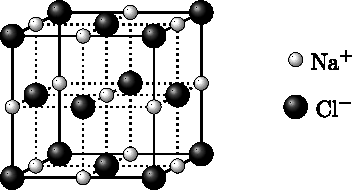
\includegraphics[width=.8\linewidth]{nacl}
	      \end{minipage}

	      \begin{tcb*}[breakable](appl)<lftt>'l'{Cristal ionique \ce{NaCl}}
		      \begin{enumerate}
			      \item Dénombrer les anions et cations dans la maille. En déduire la formule
			            brute dans la maille.
			      \item Déterminer la coordinence anions/cations.
			      \item Montrer que la structure est stable~: il y a contact entre ions de
			            charges opposées mais pas entre ions de même charge. On donne $r_{+} =
				            \SI{95}{pm}$ et $r_{-} = \SI{181}{pm}$.
		      \end{enumerate}
		      \tcblower
		      \begin{enumerate}
			      \item[b]{Formule chimique}~:
			      \psw{%
				      $8\times1/8+6\times1/12=4$ ions chlorure, et
				      $12\times1/4=4$ ions sodium dans la maille $\Ra$ \fbox{\ce{NaCl}}.
			      }%
			      \vspace{20pt}
			      \item[b]{Coordinence}~:
			      \psw{%
				      un cation a 6 anions plus proches voisins (avec qui il est en
				      contact), et 12 cations (et inversement) (on parle de structure
				      6-6).
			      }%
			      \vspace{20pt}
			      \item[b]{Stabilité}~:
			      \psw{%
			      contact entre ions de charges opposées donne $a = 2r_{+} +
				      2r_{-}$. La condition de non-contact entre deux anions d'une face
			      est $a \sqrt{2} > 4r_{-}$. Ainsi,
			      \begin{align*}
				      2r_{+}\sqrt{2} + 2r_{-}\sqrt{2} & > 4r_{-}
				      \\\Lra
				      r_{+} + r_{-}                   & > r_{-}\sqrt{2}
				      \\\Lra
				      \Aboxed{\frac{r_{+}}{r_{-}}     & > \sqrt{2}-1 = \num{0.414}}
			      \end{align*}
			      Or, $r_{+}/r_{-} \approx \num{0.52}$~: la condition est bien respectée.
			      }%
			      \vspace{20pt}
		      \end{enumerate}
	      \end{tcb*}
	\item
	      \noindent
	      \begin{minipage}[t]{.65\linewidth}
		      La structure \ce{CsCl} (chlorure de césium) est une structure
		      \textbf{cubique centrée}. En prenant le césium au centre et le chlore
		      sur les sommets, on a la géométrie suivante~:
	      \end{minipage}
	      \hfill
	      \begin{minipage}[t]{.30\linewidth}
		      \vspace{-20pt}
		      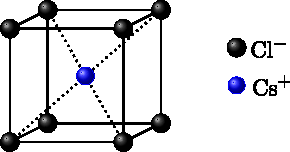
\includegraphics[width=.8\linewidth]{cscl}
	      \end{minipage}
	      % \vspace{20pt}
	      \begin{itemize}[]
		      \item[b]{Formule chimique}:
		      \psw{on a $8\times1/8 = 1$ ion chlorure,
			      et 1 ion césium dans la maille $\Ra$ \fbox{\ce{CsCl}}.}
		      \vspace{20pt}
		      \item[b]{Coordinence}:
		      \psw{un cation a 8 anions plus proches voisins (contact) et 6
			      cations, et inversement (on parle de structure 8-8).}
		      \vspace{20pt}
		      \item[b]{Stabilité}:
		      \psw{%
			      contact anion/cation sur la \textbf{grande
				      diagonale}, soit $a \sqrt{3} = 2r_{+} + 2r_{-}$, et
			      \textbf{non-contact} sur une face soit $a > 2r_{-}$~:
			      \begin{align*}
				      \frac{2}{\sqrt{3}}r_{+} + \frac{2}{\sqrt{3}}r_{-} & > 2r_{-}
				      \\\Lra
				      r_{+} + r_{-}                                     & > r_{-}\sqrt{3}
				      \\\Lra
				      \Aboxed{\frac{r_{+}}{r_{-}}                       & > \sqrt{3}-1 = \num{0.732}}
			      \end{align*}
		      }%
		      \vspace{20pt}
	      \end{itemize}
	\item
	      \noindent
	      \begin{minipage}[t]{.65\linewidth}
		      La structure \ce{ZnS} (sulfure de zinc) est une structure
		      \textbf{cubique faces centrées}. Les ions sulfure sont sur les nœuds,
		      les ions zinc sur \textbf{un site tétraédrique sur deux}.
	      \end{minipage}
	      \hfill
	      \begin{minipage}[t]{.30\linewidth}
		      \vspace{-20pt}
		      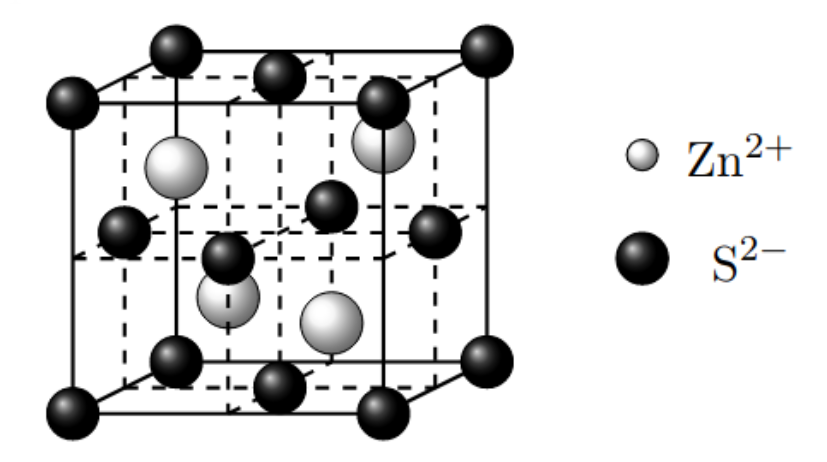
\includegraphics[width=.8\linewidth]{zns}
	      \end{minipage}
	      % \vspace{20pt}
	      \begin{itemize}[]
		      \item[b]{Formule chimique}~:
		      \psw{on a $8\times1/8 +6\times1/2 = 4$ ions sulfure,
			      et 4 ions zinc dans la maille $\Ra$ \ce{Zn4S4} ou \fbox{\ce{ZnS}}.}
		      \vspace{20pt}
		      \item[b]{Coordinence}~:
		      \psw{un cation a 4 anions plus proches voisins (contact) et 12
			      cations, et inversement (on parle de structure 4-4).}
		      \vspace{20pt}
		      \item[b]{Stabilité}~:
		      \psw{%
			      contact anion/cation sur la \textbf{grande
				      diagonale d'un petit cube}, soit $a \sqrt{3}/2 = 2r_{+} + 2r_{-}$, et
			      \textbf{non-contact} sur une face soit $a \sqrt{2} > 4r_{-}$~:
			      \begin{align*}
				      a \sqrt{2}                  & = 4 \sqrt{\frac{2}{3}}r_{+} + 4 \sqrt{\frac{2}{3}}r_{-}
				      \\\Ra
				      r_{-}                       & < r_{+}\sqrt{\frac{2}{3}} + r_{-}\sqrt{\frac{2}{3}}
				      \\\Lra
				      \Aboxed{\frac{r_{+}}{r_{-}} & > \sqrt{\frac{3}{2}}-1 = \num{0.225}}
			      \end{align*}
		      }%
	      \end{itemize}
\end{itemize}

\subsection{Cristaux covalents ou macrovalents}
\begin{tcb*}(defi){Cristal covalent}
	\psw{
		\begin{center}
			Dans un cristal macrovalent, \textbf{tous} les atomes du cristal sont liés
			entre eux par des liaisons covalentes.
		\end{center}
	}
\end{tcb*}
On trouvera ainsi principalement des éléments qui ne font peu d'ions, mais qui
font beaucoup de liaisons~: ceux avec une couche de valence environ à moitié
pleine, donc bloc d et la gauche du bloc p (carbone, silicium…).

% \begin{tcb*}(prop){Liaison covalente}
% 	\psw{
% 		\begin{center}
% 			La liaison des cristaux covalents est \textbf{très forte} ($E \gtrsim
% 			\SI{300}{kJ.mol^{-1}}$) et \textbf{directionnelle}.
% 		\end{center}
% 	}
% \end{tcb*}
%
L'étude de leurs propriétés microscopique permet d'expliquer leurs propriétés
macroscopiques~:
\begin{tcb*}[tabularx={lXcY}, label=ror:ptemet](ror){Propriétés des cristaux
			covalents}
	\\[-0.5em]
	\textbf{Type}                                                                        &
	\multicolumn{1}{Y}{%
		\textbf{Ppté.\ microscopique}}                                                       &       &
	\textbf{Ppté.\ macroscopique}
	\\\midrule
	\textbf{Mécanique}                                                                   &
	Liaison directionnelle, atomes fixes                                                 & $\Ra$ &
	\psw{grande dureté}
	$\xmathstrut{\rght}$
	\\\midrule
	\textbf{Thermique}                                                                   &
	Liaison covalente très forte\ftn{$\Ec\ind{covalente} \approx \SI{300}{kJ.mol^{-1}}$} & $\Ra$ &
	\psw{température de fusion très élevée}
	$\xmathstrut{\rght}$
	\\\midrule
	\textbf{Électrique}                                                                  &
	Électrons localisés dans les liaisons                                                & $\Ra$ &
	\psw{isolant électrique}
	$\xmathstrut{\rght}$
	\\\bottomrule
\end{tcb*}

\begin{tcb*}(appl)<lftt>'l'{Cristal covalent}
	\begin{wrapfigure}[4]{R}{.2\linewidth}
		\vspace*{-20pt}
		\centering
		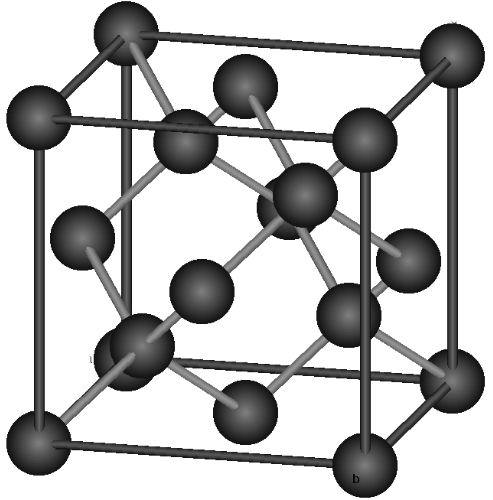
\includegraphics[width=.8\linewidth]{maille_diamant}
	\end{wrapfigure}
	Le cas du carbone diamant est un cristal covalent, qui forme un réseau CFC
	avec la moitié des sites tétraédriques également occupés par des atomes de
	carbone.
	\begin{enumerate}
		\item Déterminer sa compacité.
		\item Déterminer sa masse volumique. On donne $a = \SI{356.7}{pm}$.
	\end{enumerate}
	\tcblower
	\psw{%
		\begin{enumerate}
			\item Contact sur la grande diagonale d'un petit cube~: $a \sqrt{3}/2 =
				      4r$. Or, on compte $4+6\times1/2+8\times1/8 = 8$ atomes par maille.
			      Ainsi,
			      \begin{align*}
				      C         & = \frac{NV\ind{sph}}{V\ind{m}}
				      \\\Lra
				      C         & = \frac{8\times \frac{4}{3}\pi r^3}{a^3}
				      \\\Lra
				      C         & = \frac{\frac{32}{3}\pi r^3}{\frac{512}{3 \sqrt{3}}r^3}
				      \\\Lra
				      \Aboxed{C & = \frac{\pi \sqrt{3}}{16} \approx \num{0.34}}
			      \end{align*}
			\item La masse volumique, avec $M_{\ce{C}} = \SI{12}{g.mol^{-1}}$, est
			      \[
				      \boxed{
					      \rho = \frac{NM}{\Nc_Aa^3} \approx \SI{3500}{kg.m ^{-3}}
				      }
			      \]
		\end{enumerate}
	}%
	\vspace{-15pt}
\end{tcb*}

\begin{tcb}(rema)<lftt>{Graphite et diamant}
	Le graphite est formé d'atomes de carbone disposés en plans parallèles. La
	cohésion entre les différents plans est assurée par des liaisons de
	\textsc{van Der Waals}, ce qui fait que les différents plans peuvent
	facilement «~glisser~» les uns sur les autres, et donc être déposés sur une
	feuille par les mines de crayon.
	% Les plans sont organisés en hexagones et le plan du dessus est décalé par
	% rapport au plan du dessous.
\end{tcb}

\subsection{Cristaux moléculaires}
\begin{tcb*}(defi){Cristal moléculaire}
	\psw{
		\begin{center}
			Un cristal moléculaire est fait de \textbf{molécules} liées entre elles
			par des \textbf{liaisons de \textsc{vdW}} ou \textbf{liaisons hydrogènes}.
		\end{center}
	}
\end{tcb*}
Le modèle des sphères dures n'est pas toujours adapté dans ce cas, puisque leur
géométrie est souvent anisotrope~: les motifs sont \textbf{orientés} dans la
maille, de telle sorte qu'ils maximisent l'énergie de liaison.

% \begin{tcb*}(prop){Liaison moléculaire}
% 	\psw{
% 		\begin{center}
% 			La liaison des cristaux moléculaires est \textbf{faible} ($E \lesssim
% 			\SI{10}{kJ.mol^{-1}}$ pour VdW, $\approx \SI{30}{kJ.mol^{-1}}$ pour les
% 			LH) et \textbf{directionnelle}.
% 		\end{center}
% 	}
% \end{tcb*}

L'étude de leurs propriétés microscopique permet d'expliquer leurs propriétés
macroscopiques~:
\begin{tcb*}[tabularx={lXcY}, label=ror:ptemol](ror){Propriétés des cristaux moléculaires}
	\\[-0.5em]
	\textbf{Type}                                      &
	\multicolumn{1}{Y}{%
		\textbf{Ppté.\ microscopique}}                     &       &
	\textbf{Ppté.\ macroscopique}
	\\\midrule
	\textbf{Mécanique}                                 &
	Liaison directionnelle mais faible donc déplaçable & $\Ra$ &
	\psw{faible dureté}
	\\\midrule
	\textbf{Thermique}                                 &
	Liaisons VdW et LH faibles\ftn{%
		$\Ec\ind{\textsc{vdW}} \lesssim \SI{10}{kJ.mol^{-1}}$ et
		$\Ec\ind{LH} \approx \SI{30}{kJ.mol^{-1}}$.}       & $\Ra$ &
	\psw{faibles températures de fusion/ébullition}
	\\\midrule
	\textbf{Électrique}                                &
	Électrons localisés dans les molécules
	$\xmathstrut{\rght}$
	& $\Ra$ &
	\psw{isolant électrique}
	\\\midrule
	\textbf{Chimique}                                  &
	Interac$^\circ$ intérieures similaires aux solvants   & $\Ra$  &
	\psw{forte solubilité si solvant adapté}
	\\\bottomrule
	% \begin{center}
	% 	\renewcommand\arraystretch{1.6}
	% 	\captionof{table}{Propriétés des cristaux moléculaires}
	% 	\label{tab:ptemol}
	% 	\begin{tabularx}{\linewidth}{lXcY}
	% 		\toprule
	% 		\textbf{Type}                                      &
	% 		\multicolumn{1}{Y}{%
	% 		\textbf{Ppté.\ microscopique}}                     &       &
	% 		\textbf{Ppté.\ macroscopique}
	% 		\\\midrule
	% 		\textbf{Mécanique}                                 &
	% 		Liaison directionnelle mais faible donc déplaçable & $\Ra$ &
	% 		\psw{faible dureté}
	% 		\\\midrule
	% 		\textbf{Thermique}                                 &
	% 		Liaisons VdW et LH faibles\ftn{%
	% 			$\Ec\ind{\textsc{vdW}} \approx \SI{10}{kJ.mol^{-1}}$ et
	% 		$\Ec\ind{LH} \approx \SI{30}{kJ.mol^{-1}}$.}       & $\Ra$ &
	% 		\psw{faibles températures de fusion/ébullition}
	% 		\\\midrule
	% 		\textbf{Électrique}                                &
	% 		Électrons localisés dans les molécules             & $\Ra$ &
	% 		\psw{isolant électrique}
	% 		\\\midrule
	% 		\textbf{Chimique}                                  &
	% 		Interactions intérieures similaires aux solvants   & donc  &
	% 		\psw{forte solubilité si solvant adapté}
	% 		\\\bottomrule
	% 	\end{tabularx}
	% \end{center}
\end{tcb*}

\begin{tcb}[sidebyside, righthand ratio=.3](exem)<lftt>{Cristal moléculaire}
	Ce sont souvent ces solides que l'on manipule en TP, le plus courant étant
	bien entendu l'eau sous forme de glace. On montre ci-contre la structure
	moléculaire de la glace I. La cohésion est assurée par les liaisons hydrogène.
	\tcblower
	\begin{center}
		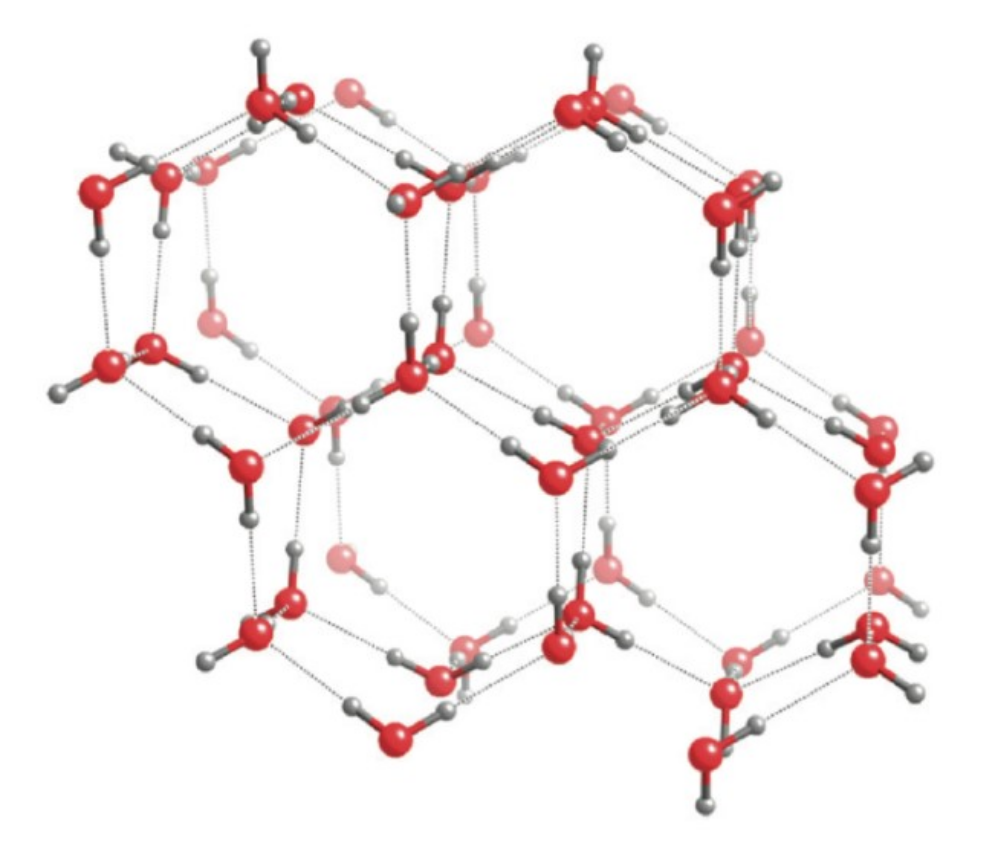
\includegraphics[width=\linewidth]{crist_mol_exem}
	\end{center}
\end{tcb}

\def\rght{1.00}
\subsection{Bilan}
\begin{table}[h!]
	\footnotesize
	\renewcommand\arraystretch{2.0}
	\begin{center}
		\caption{Bilan des différents types de cristaux.}
		\label{tab:bilan}
		\begin{tabularx}{\linewidth}{lYYYY}
			\toprule
			                                                        &
			\textbf{Cristaux métalliques}                           &
			\textbf{Cristaux ioniques}                              &
			\textbf{Cristaux covalents}                             &
			\textbf{Cristaux moléculaires}
			\\\cmidrule(lr){2-5}
			\textbf{Exemples}                                       &
			\ce{Fe}, \ce{Ca}, \ce{Zn}                               &
			\ce{NaCl}, \ce{KOH}                                     &
			Diamant, \ce{Si}, \ce{Ge}                               &
			\ce{H2O}, \ce{I2}, \ce{CO2}
			$\xmathstrut{\rght}$
			\\\midrule
			\textbf{Liaison}                                        &
			\psw{Métallique (é.\ délocalisés)}                      &
			\psw{Ionique (entre + et $-$)}                          &
			\psw{Covalente}                                         &
			\psw{VdW, LH}
			$\xmathstrut{\rght}$
			\\\midrule
			\textbf{Mécanique}                                      &
			\psw{Dur, malléable, ductile}                           &
			\psw{Dur mais cassant}                                  &
			\psw{Dur et peu malléable}                              &
			\psw{Fragile}
			$\xmathstrut{\rght}$
			\\\midrule
			$\mathbf{T\ind{fus}}$                                   &
			\psw{Élevée ($\approx \SI{e3}{\degreeCelsius}$) }       &
			\psw{Assez élevée ($\approx \SI{e2}{\degreeCelsius}$) } &
			\psw{Élevée ($\approx \SI{e3}{\degreeCelsius}$) }       &
			\psw{Faible ($\lesssim \SI{100}{\degreeCelsius}$)}
			$\xmathstrut{\rght}$
			\\\midrule
			\textbf{Électrique}                                     &
			\psw{Conducteur}                                        &
			\psw{Isolant}                                           &
			\psw{Le plus souvent isolant}                           &
			\psw{Isolant}
			$\xmathstrut{\rght}$
			\\\midrule
			\textbf{Solubilité}                                     &
			\psw{Insoluble}                                         &
			\psw{Très solubles dans polaires}                       &
			\psw{Insoluble}
			$\xmathstrut{\rght}$                                    &
			\psw{Très solubles si adéquat}
			\\\bottomrule
		\end{tabularx}
	\end{center}
\end{table}

\end{document}
